Here we introduce a few Poncelet triangle families interscribed in non-concentric, axis-parallel (NCAP) ellipse pairs. In some of the families below, at least one of the ellipses is a circle, so perhaps ``co-axial'' could also be employed.

\section{Poristic Family (Bicentric Triangles)}
\label{sec:04-poristic}

\begin{figure}
    \centering
    %\includegraphics[width=\textwidth]{pics/0010x_obtuse_poristics.eps}
    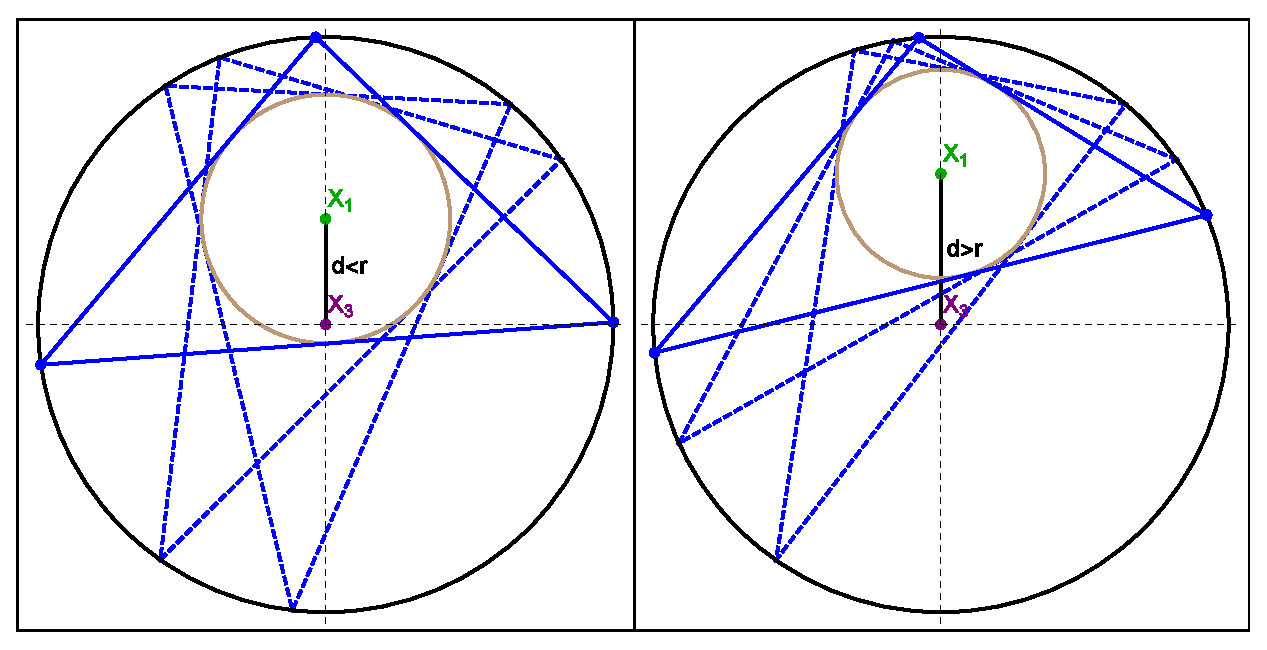
\includegraphics[width=\textwidth]{pics_04_180_obtuse_poristics}
    \caption{Poristic Triangle family (blue): fixed incircle (green) and circumcircle (purple). \textbf{Left}: a few poristic triangles (blue and dashed blue) in a pair of circles such that $d<r$, i.e.,  all poristic triangles are acute. \textbf{Right}: the same but with $d>r$; since $X_3$ can be either interior or exterior to the family, both acute and obtuse triangles will be present. \href{https://bit.ly/3bg19iD}{Live}}
    \label{fig:04-poristic obtuse}
\end{figure}

Poristic triangles, shown in \cref{fig:04-poristic obtuse}, are the simplest case of Poncelet's porism: a 1d family of triangles with fixed incircle and circumcircle. They are also known as the ($N=3$) bicentric family.

First described by \cite{chapple1746-poristics}, the family was later studied by both Euler and Poncelet. The so-called Euler's triangle formula\footnote{Chapple had stated it in 1746, Euler in 1765, and Poncelet's porism was published in 1822; see \cite{centina15}.}, constrains the distance $d$ between incenter $X_1$ and circumcenter $X_3$ as follows:

\begin{equation}
d^2=R(R-2 r)
\label{eq:04-euler-poristic}
\end{equation}
where $r,R$ are the radii of outer and inner circle. Referring to \cref{fig:04-poristic obtuse}:

\begin{proposition}
The Poristic family will contain obtuse triangles iff $d>r$.
\end{proposition}

\begin{proof}
This stems from the fact that when $d<r$, $X_3$ is always interior to the incircle, i.e., the caustic of the Poncelet family. 
\end{proof}

In consonance with both billiard 3-periodics and the incircle family:

\begin{proposition}
The poristic family conserves the sum of its internal angle cosines.
\end{proposition}

\begin{proof}
Direct application of \cref{eqn:02-sum-cos}, noting by definition $r/R$ is constant.
\end{proof}

\begin{figure}
    \centering
    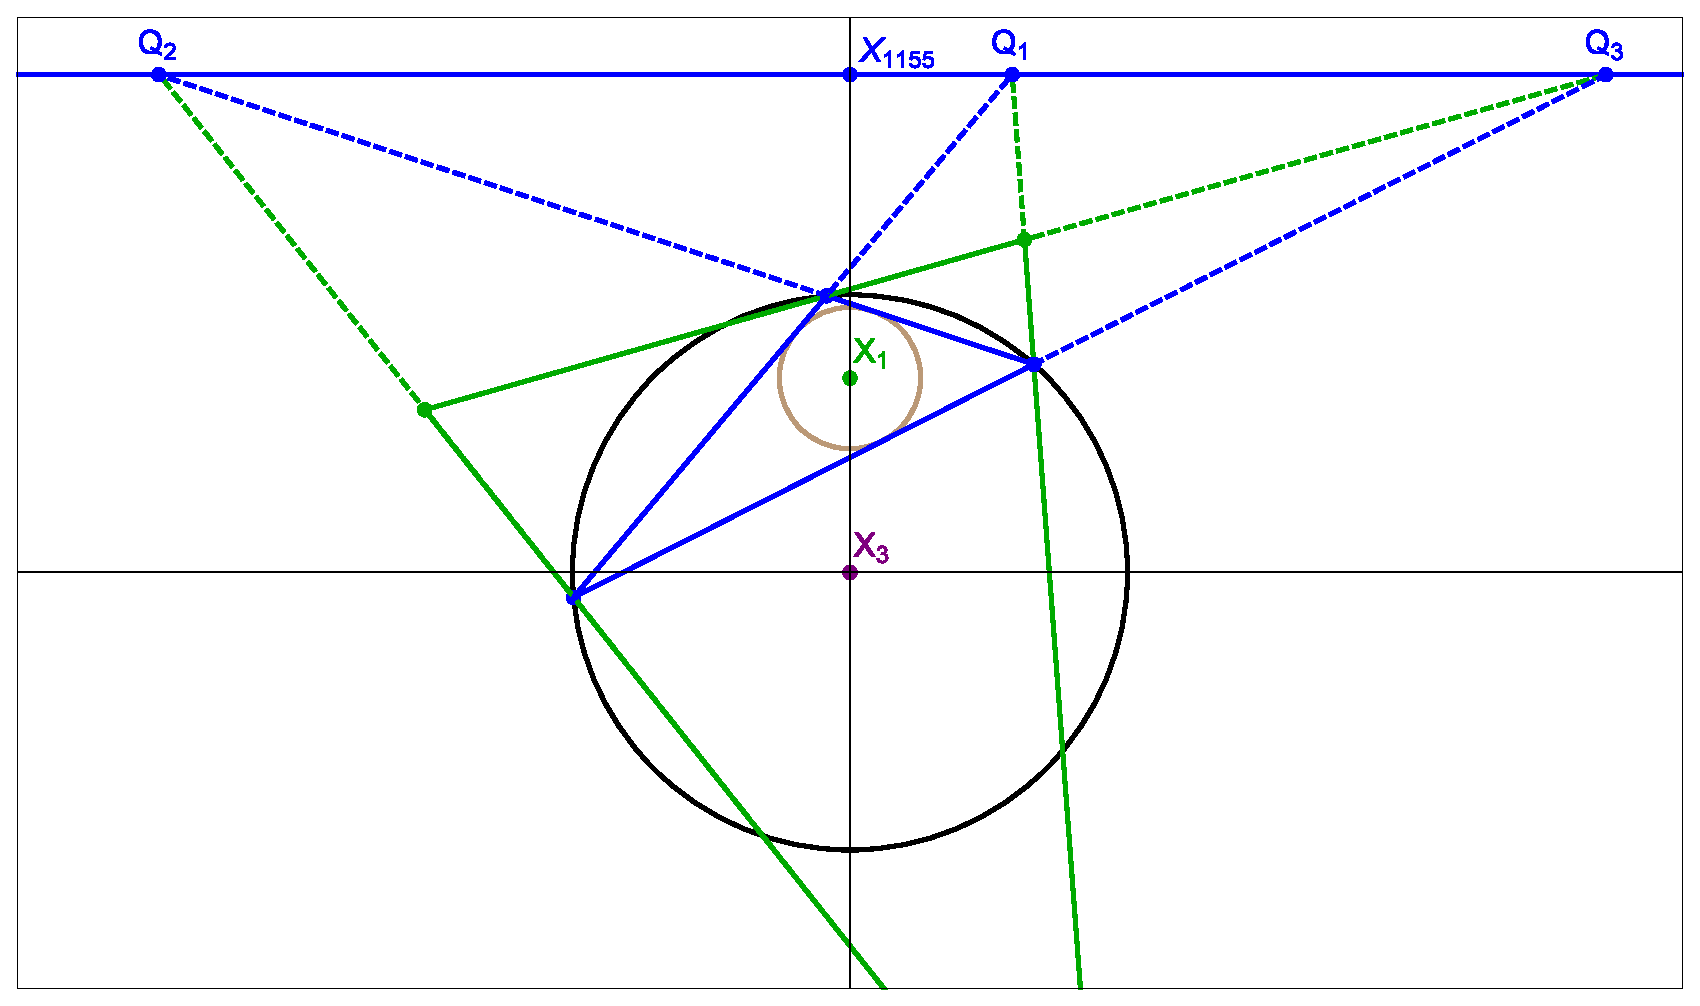
\includegraphics[width=.7\textwidth]{pics_04_220_poristic_antiorthic}
    \caption{Over the poristic family, the antiorthic axis (solid blue) is stationary and perpendicular to $X_1 X_3$. \href{https://youtu.be/DS4ryndDK6Q}{Video}.}
    \label{fig:04-antiorthic}
\end{figure}

In \cite[Antiorthic axis]{mw} the anti-orthic axis is defined as containing the three intersections of a triangle's sidelines with those of the excentral triangle. As illustrated in \cref{fig:04-antiorthic}, the following was proved by \cite{weaver1927-poristic}:

\begin{proposition}
The antiorthic family is stationary over the poristic family and perpendicular to $X_1 X_3$.
\label{prop:04-antiorthic}
\end{proposition}

Let a first vertex $P_1$ of the poristic family be parametrized by $P_1(t)=R[\cos{t},\sin{t}]$.

\begin{proposition}
The perimeter $L(t)$ of poristic triangles is given by:

\begin{equation*}
L(t)=\frac {\left(3\,{R}^{2}
-4\,dR\cos t  +{d}^{2} \right)\sqrt{3\,{R}^{2}+2\,dR\cos t  -{d}^{2}}  }{R\sqrt {{R}^{2}-2\,dR
\cos t  +{d}^{2}}}\\
\end{equation*}
\end{proposition}
\begin{proof}
Follows directly computing the 3-vertices explicitly and using $L(t)=|P_1-P_2|+|P_2-P_3|+|P_3-P_1|$ and simplifying it with a CAS.  
\end{proof}

It turns out poristic triangles can be regarded as the image of billiard 3-periodics (and vice-versa) under (i) a variable similarity transform, and (ii) a polar transformation wrt to a focus-centered circle. We now proceed to prove these results, but first we will need a couple of lemmas.

In \cite[page 17]{odehnal2011-poristic}, one finds the following result, illustrated in \cref{fig:04-poristic-x9}:

\begin{figure}
    \centering
    %\includegraphics[width=.8\textwidth]{pics/0050x_poristic_cb.eps}
    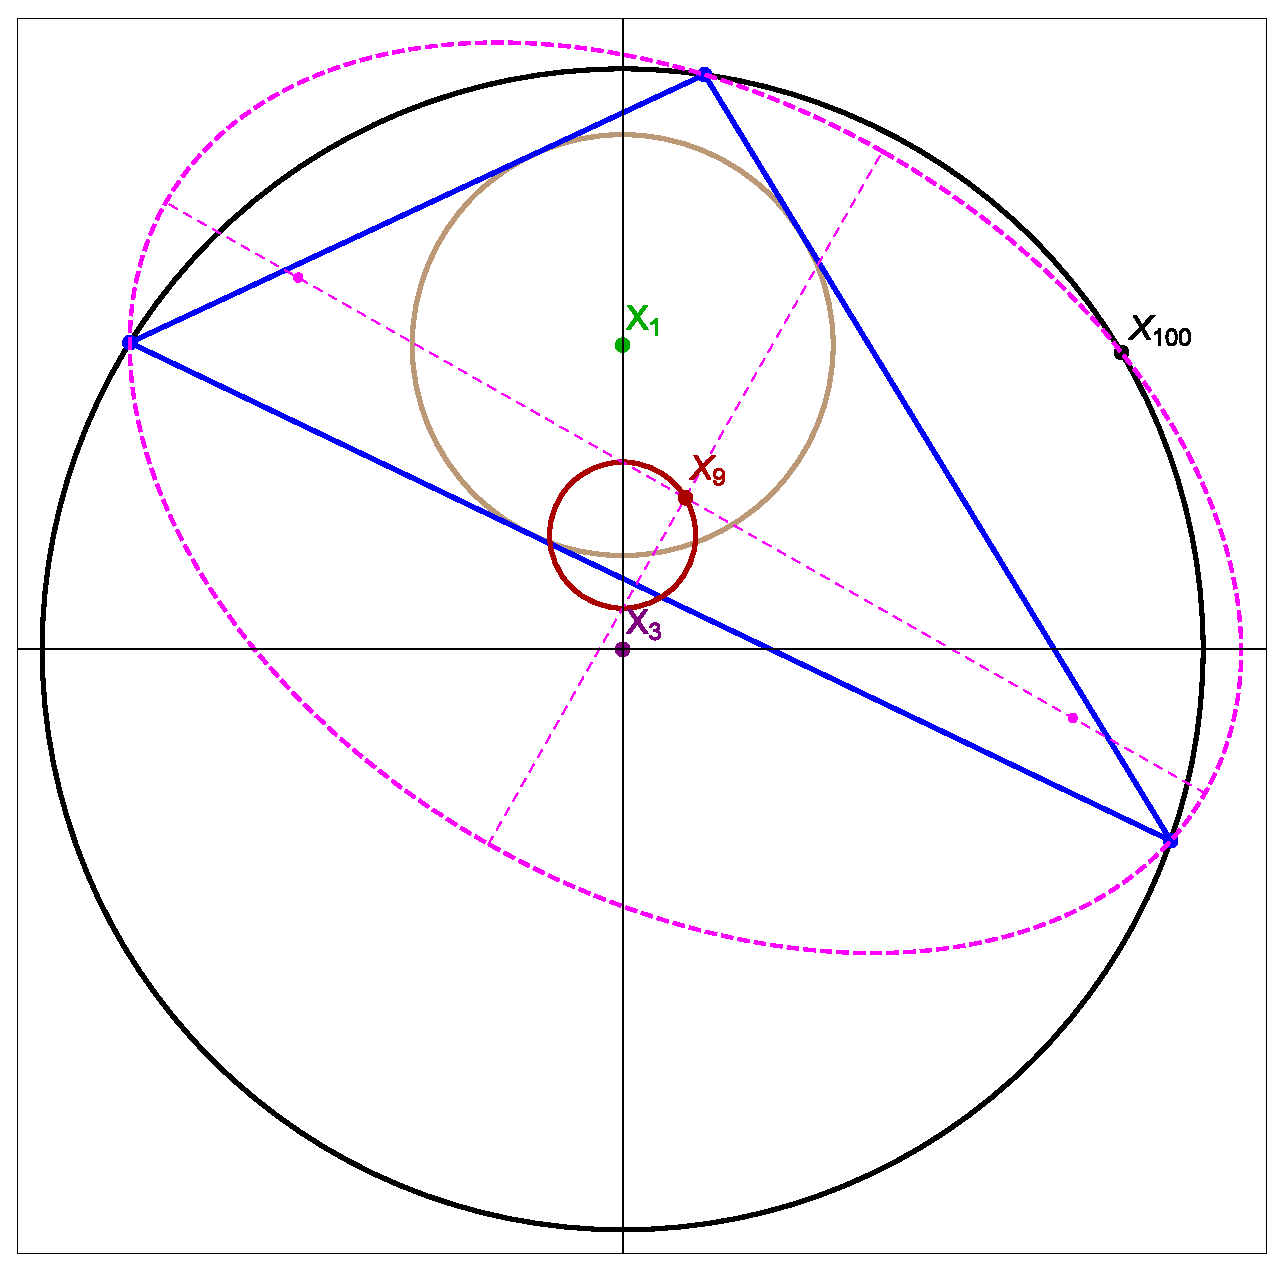
\includegraphics[width=.8\textwidth]{pics_04_190_poristic_cb}
    \caption{A poristic triangles (blue) is shown along as its circumbilliard (dashed magenta) whose aspect ratio is invariant. The locus of the mittenpunkt $X_9$ is a circle (red). \href{https://youtu.be/LGgh11LMGGY}{Video}, \href{https://bit.ly/3tcGtOj}{Live}}
    \label{fig:04-poristic-x9}
\end{figure}

\begin{lemma}
Over the poristic family, the locus of the mittenpunkt $X_9$ is a circle with radius is $R{d^2}R/(9R^2-d^2)$ centered on $X_1 + (X_1 - X_3) (2 R - r)/(4 R + r)=d (3 R^2+d^2)/(9R^2-d^2)$. 
\end{lemma}

In fact we can derive $X_9(t)$ explicitly:

\begin{lemma}
{\small
\begin{align}
    X_9(t)= &\left[  \frac {d \left( 4\, d \mathbf{c}^2   
 \left( R\mathbf{c}_t-d \right) -r \left( 3\,d\mathbf{c}_t  +R \right) -{r}^{2} \right) }{ \left( 4\,R+r \right) 
 \left(d \mathbf{c}_t  -R+r \right) }
  , \, \frac {4R{d}^{2}\mathbf{s}_t  \left( R^2- \left( 2\,R\mathbf{c}_t-d \right) ^{2}  \right) }{ \left( {R}^{2}+{d
}^{2}-2\,dR\mathbf{c}_t  \right)  \left( 9\,{R}^{2}-{d}^{2}
 \right) }
    \right]
\label{eq:04-x9-poristic}
\end{align}
where $\mathbf{c}_t$ and $\mathbf{s}_t$ are shorthand for $\cos(t)$ and $\sin(t)$ respectively.
}
\end{lemma}

Let $P_i=[x_i,y_i]$ denote the vertices of billiard 3-periodics and $P_i'=[x_i',y_i']$ those of a poristic family, $i=1,2,3$.

\begin{theorem}
The $P_i'$ are an image of the $P_i$ under a variable similarity transform comprising of (i) a rigid rotation by $\theta(t)$, (ii) a rigid translation by $X_9(t)$, and (iii)  uniform scaling by $L(t)$. These are given by: 

\begin{align*}
    x_i'=&L(t)(\cos \theta(t) x_i+\sin\theta(t) y_i+x_9(t) )\\
    y_i'=&L(t)(-sin\theta(t) x_i+\cos\theta(t) y_i+y_9(t))\\
    \tan\theta(t)=& \frac{(1-\cos t)(R+d-2R\cos t)}{(2R\cos t+R-d)\sin t}
\end{align*}
\label{thm:similarity}
\end{theorem}

\begin{proof} 
CAS-assisted simplification.
\end{proof}

In \cite{reznik2021-circum} term the ``circumbilliard'' $E_9$ of a triangle the circumellipse centered on $X_9$. Let $a_9,b_9$ its semi-axes. CAS manipulation yields:

\begin{corollary}
Over the poristic family, $a_9(t)$ and $b_9(t)$ are given by:
\begin{align*}
a_9=&L(t)\frac{R\sqrt {3\,{R}^{2}+2\,dR-{d}^{2}} }{9\,{R}^{2}-{d}^{2}}\\
b_9=&  L(t)\frac{R\sqrt {R-d}}{\sqrt {3\,R+d} (3\,R-d)}\\
  c_9=&\sqrt{a_9^2-b_9^2}=L(t)\frac{2R\sqrt{dR}}{9R^2-d^2}.
\end{align*}
\end{corollary}

\begin{corollary}
The ratios $a_9(t)/L(t)$, $b_9(t)/L(t)$, and $c_9(t)/L(t)$ are invariant over the Poristic family.
\end{corollary}

\begin{corollary}
Over the poristic family, the aspect ratio of the (varying) circumbilliard is invariant and given by:

\begin{equation*}
\frac{a_9(t)}{b_9(t)}=\sqrt{\frac { \left(  R+d \right)  \left( 3R-d \right) }{ \left( R-d
 \right)  \left( 3\,R+d \right) }}
\end{equation*}
\end{corollary}

In \cite[Polar]{mw}, the {\em polar} of a point $P$ with respect to a circle $\Cm$ is defined as the line perpendicular to $O P$ which contains the inversion of $P$ wrt to $\Cm$. Dually, the pole of a line $L$ with respect to $\Cm$ is the inversion of the foot of the perpendicular dropped from $O$ onto $P$ wrt to $\Cm$.

So given a smooth curve, we can speak of its {\em polar image} with respect to a circle as the set of poles of the curve's tangents with respect to $\Cm$. 

\begin{figure}
    \centering
    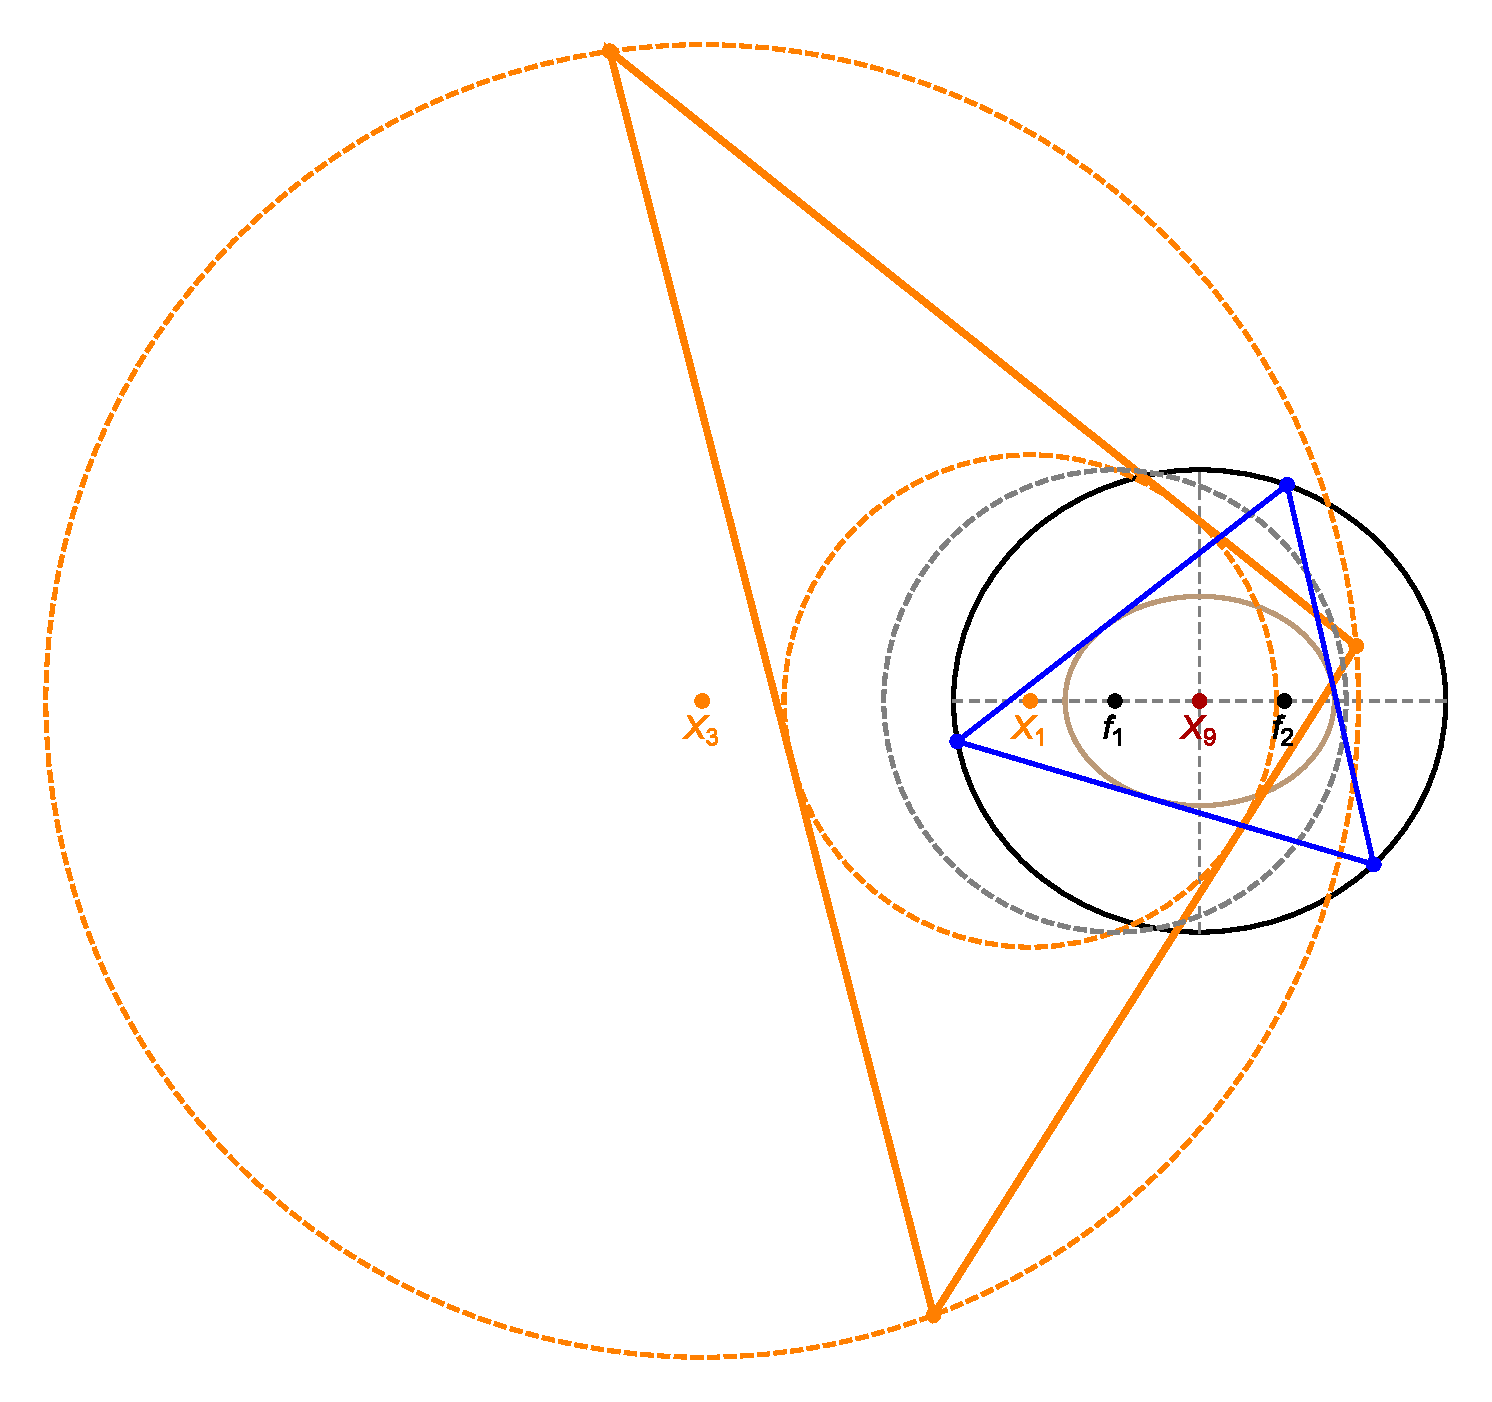
\includegraphics[width=.8\textwidth]{pics_04_200_polar_poristic}
    \caption{The poristic family (orange) is the polar image of billard 3-periodics (blue) with respect to a circle (dashed gray) centered on one of the foci of the confocal pair ($f_1$ in the picture). \href{https://bit.ly/3nQ2wcH}{Live}}
    \label{fig:04-polar-poristic}
\end{figure}

The fact that the polar image of an ellipse with respect to a focus is a circle is a well-known result \cite{akopyan2007-conics}.

Let $\E$ and $\E'$ be a confocal ellipse pair centered at $[0,0]$, with major axes along $x$. Let $a,b$ and $a',b'$ denote their major and minor semi-axes, respectively. The foci $f_1$ and $f_2$ are at $[\pm c,0]$, where $c^2=a^2-b^2$. A known classical result which we reproduce below is:

\begin{lemma}
The polar image of the $\E,\E'$ pair with respect to a circle of radius $\rho$ centered on $f_1$ is a pair of nested circles $\Cm_{int},\Cm_{ext}$ with centers given by:

\[\Om_{int}=[-c-\rho^2\frac{c}{b^2},0],\;\;\;\Om_{ext}=[-c-\rho^2\frac{c}{b'^2},0]\]
Their radii $r,R$ and distance $d$ between their centers are given by: 

\[ r=\rho^2\frac{a}{b^2},\;\;\;R=\rho^2\frac{a'}{b'^2},\;\;\; d=\rho^2\frac{ c\, (a^2 - {a'}^2)}{b^2\, {b'}^2} \]
\end{lemma}

%Recall also that a pair of circles uniquely is defines a {\em pencil} of coaxial circles; see \cite[Limiting Points]{mw}. The pencil contains exactly two circles which degenerate to a point, known as {\em limiting points}. A known result is:

%\begin{lemma}
%The limiting points $\ell_1,\ell_2$ of the polar image of a confocal pair $\E,\E'$ with respect to a $f_1$-centered circle are located at $f_1=[-c,0]$ and $[-c+\frac{\rho^2}{c},0]$.
%\end{lemma}
 
Referring to \cref{fig:04-polar-poristic}:

\begin{corollary}
The poristic family is the polar image of billiard 3-periodics with respect to a circle centered on a focus. 
\label{cor:04-poristic-polar-image}
\end{corollary}

\begin{corollary}
The sum of cosines of the polar image of billiard 3-periodics with respect to a focus-centered circle is given by:

\begin{equation}
\sum\cos\theta' = 1+\frac{r}{R} = 1+\frac{a b'^2}{a' b^2}
\label{eq:04-bic-cos}
\end{equation}
\end{corollary}

\begin{figure}
    \centering
    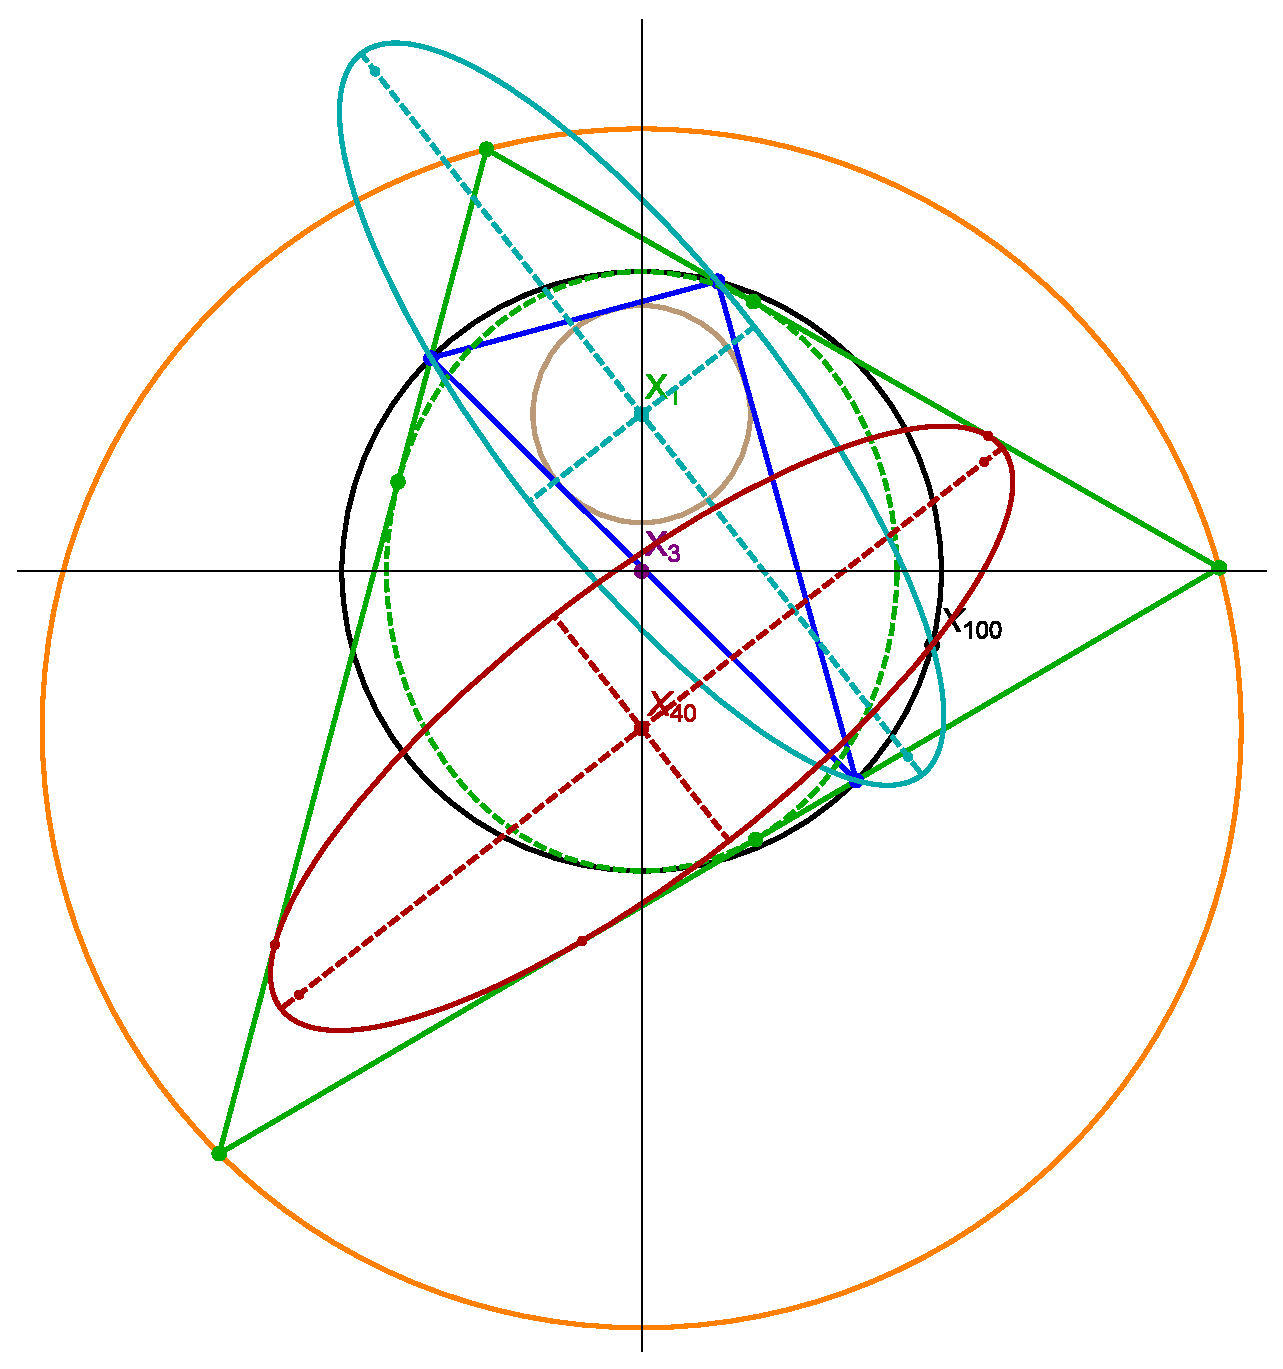
\includegraphics[width=.7\textwidth]{pics_04_230_excentral_poristic_inconics}
    \caption{A poristic triangle (blue) is shown, as well as $I_1$, the $X_1$-centered inconic (light blue). Also shown is the excentral triangle (green), the circle (orange) the excentral family is inscribed in and their MacBeath caustic (dashed green). Also shown is $I_3'$ (dark red), the $X_3'$-centered excentral inconic (red). Note $X_3'=X_{40}$. Over the poristic family, both $I_1$ and $I_3'$ rotated rigidly at 90-degrees from each other. \href{https://youtu.be/hz0qEyVVvaI}{Video}}
    \label{fig:04-excentral-poristic-inconics}
\end{figure}

Given a triangle, an inconic is is fully defined by its center and is tangent to the three sidelines, see \cite[Inconic]{mw}.

Referring to \cref{fig:04-excentral-poristic-inconics}, let $E_1$ be the $X_1$-centered circumconcic to the poristic family, i.e., it contains the vertices. Let $\mu_1$, and $\nu_1$ denote its semi-axes. Interestingly:

\begin{proposition}
$\mu_1=R+d$ and $\nu_1=R-d$ are invariant over the poristic family, i.e., $E_1$ rigidly rotates about $X_1$. \label{prop:04-e1}
\end{proposition}

A proof appears in \cite[Appendix C]{garcia2020-similarity-I}.
\section{Poristic Excentrals}

\begin{figure}
    \centering
    %\includegraphics[width=.7\textwidth]{pics/0170_poristic.eps}
    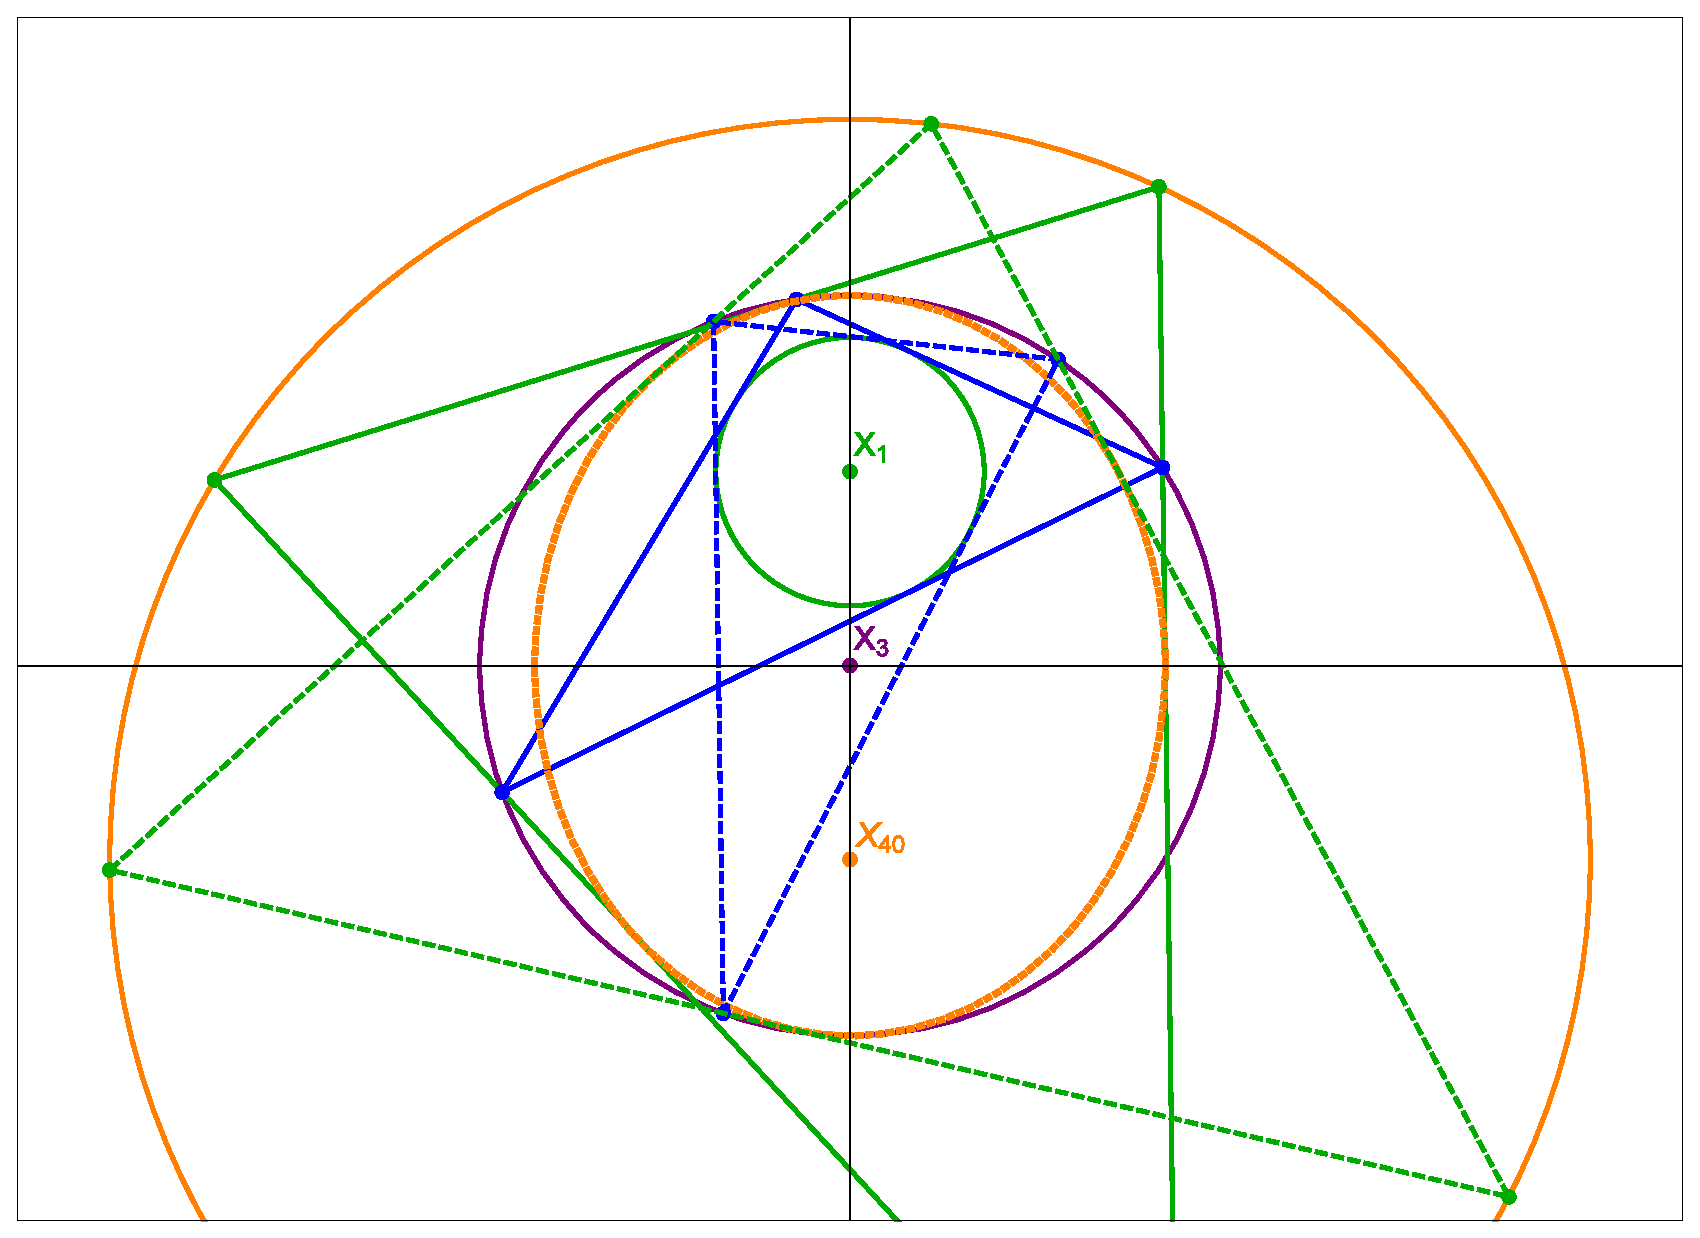
\includegraphics[width=\textwidth]{pics_04_170_poristic}
    \caption{The poristic family (blue) is interscribed between two fixed circles, i.e., their circumcenter $X_3$ and incenter $X_1$ are stationary. The family of its excentral triangles (solid green) are inscribed in a circle (orange) centered on the Bevan point $X_{40}$ and of radius twice the original circumradius. This family circumscribes the MacBeath inellipse (dashed orange), centered on $X_3$ with foci on $X_1$ and $X_{40}$. A second for both poristics and excentrals configuration is also shown (dashed blue and dashed green).  \href{https://youtu.be/DS4ryndDK6Q}{Video}, \href{https://bit.ly/2RoYJHm}{Live}}
    \label{fig:04-poristic-excentrals}
\end{figure}

The family of excentral triangles to the poristic family, shown in \cref{fig:04-poristic-excentrals} is also Ponceletian: in \cite{odehnal2011-poristic}, it is shown to be inscribed in a circle of radius $2R$ where $R$ is the circumradius of its reference poristic family, centered on $X_{40}$, the Bevan point, or $X_3'$ of the family in questions (to avoid confusion, we will be priming quantities associated with this family).

\begin{proposition}
The barycenter $X_2'$ of poristic excentrals is stationary.
\end{proposition}

\begin{proof}
Recall a triangle's barycenter $X_2$ is a third of the way from the circumcenter to the orthocenter \cite[Euler Line, Eqn. 6]{mw}. The result follows from the fact that both $X_3'=X_{40}$ and $X_4'=X_1$ are stationary.
\end{proof}

The MacBeath inconic, defined in \cite[MacBeath Inconic]{mw}, is an ellipse centered on a triangle's 9-point center $X_5$, with  foci at the circumcenter $X_3$ and orthocenter $X_5$.

Poristic excentrals are Ponceletian since:

\begin{proposition}
The MacBeath inconic to the excentral poristics is stationary and is therefore the caustic. Let $\mu_5'$ and $\nu_5'$ denote its major and minor semi-axes. These are given by:
\[ \mu_5'=R,\;\;\;\nu_5'=\sqrt{R^2-d^2} \]
\end{proposition}

\begin{proof}
It is straightforward to verify the sidelines of poristic excentrals are dynamically  tangent to the ellipse:
\[
\frac{(x-d)^2}{R^2}+\frac{y^2}{R^2-d^2}=1\]
with center $X_3=(d,0)$ and foci $X_{40}=(0,0)$ and $X_1=(2d,0)$.
\end{proof}

Correspondences between the centers and foci of the excentral MacBeath inconic and those of the reference triangle appear in \cref{tab:04-macbeath}.

\begin{table}
\centering
\begin{tabular}{|c|c|c|}
\hline
\makecell[cc]{excentral\\ MacBeath} &
\makecell[cc]{excentral\\center} &
\makecell[cc]{reference\\center} \\
\hline
center & $X_5'$ & $X_3$\\
focus & $X_4'$ & $X_1$  \\
focus & $X_3'$ & $X_{40}$ \\
\hline
\end{tabular}
\caption{Center and foci of the MacBeath inconic of an excentral triangle and the corresponding triangle center of the reference.} 
\label{tab:04-macbeath}
\end{table}

Since $\mu'_5/\nu_5'=R/\sqrt{R^2-d^2}$, use \cref{eq:04-euler-poristic} to obtain:

\begin{corollary}
The aspect ratio of the caustic to the excentral poristics is given by:
\begin{equation*}
 \frac{\mu'_5}{\nu_5'}={\sqrt\frac{R}{2 r}}
\end{equation*}
\end{corollary}

As shown in \cref{fig:04-excentral-poristic-inconics}, let $I_3'$ be the $X_3'$-centered inconic to poristic excentrals. Let $\mu_3'$ and $\nu_3'$ denot its major and minor semi-axes, respectively.

\begin{proposition}
Over poristic excentrals,  $\mu_3'=R+d$ and $\nu_3'=R-d$ are invariant, i.e., $I_3'$ rigidly rotates about $X_3'$.
\label{prop:04-inconic-x3p}
\end{proposition}

We omit the long proof kindly contributed by B. Odehnal and appearing in \cite[Appendix C]{garcia2020-similarity-I}.

Interestingly:

\begin{theorem}
Excentral poristics are the image of the circumcircle family under a variable rigid rotation. The ridigly-rotating $I_3'$ is identified with the caustic of the circumcircle family.
\end{theorem} 

\begin{proof}
Recall \cref{prop:03-circumcircle-rh}: the orthic triangles of the circumcircle family has invariant inradius and circumradius. Also recall \cref{lem:03-circum-x5-locus}: the locus of the orthic circumcenter is a circle concentric with the common center. Also notice in the circumcircle family, the caustic is the stationary inconic centered on $X_3$.
\end{proof}

\section{The Brocard Porism}
 
A property-rich family of Poncelet triangles is the so-called ``Brocard porism'', introduced in  \cite{bradley2007-brocard,shail1996-brocard, bradley2011-brocard}. It is inscribed in a circle and circumscribes the so-called {\em Brocard inellipse}. Remarkably, its foci coincide with the stationary Brocard points $\Omega_1$ and $\Omega_2$ of the family; see \cref{fig:04-brocard-porism}.

Let $R$ denote the radius of the outer circle and $a',b'$ the caustic semi-axes, with $(c')^2=(a')^2-(b')^2$. Let also, $d=|X_{3}-X_{39}|$ the distance between the centers of the circle and of the caustic.

\begin{proposition}
A pair of circle (outer) $(x-x_0)^2+y^2=R^2$ and ellipse (caustic) $(x-x_1)^2/(a')^2+y^2/(b')^2=1$ admit a 1d family of Poncelet triangles if and only if 
\[(a')^2  - 2 R a'- (b')^2 +  R^2-d^2=0,\;\; d=|x_1-x_0| \]
\end{proposition}
\begin{proof}
  Follows from Cayley condition for 3-periodics in an NCAP pair.
  %\textcolor{red}{citar prop. cap 2}
\end{proof}
\begin{proposition}
For any triangle $T$, the circumcircle and Brocard inellipse are Ponceletian, they admit a 1d family of Poncelet triangles. Furthermore, their Brocard inellipse is stationary.
\label{prop:04-broc-inellipse-stationary}
\end{proposition}

\begin{proof}
Follows from vertex parametrization for the Brocard family and/or from stationarity of $X_6$, see \cref{prop:03-x6-stationary}. 
\end{proof}

\begin{proposition}
The stationary circumcenter $X_3$ and circumradius $R$ are given by:

\begin{equation}
X_3=[0,-\frac{c'\delta_1}{b'}],\;\;\;R= \frac{2 (a')^2}{b'} \\
 %=& \frac{\sqrt{3a^2+2c^2-2c\delta_1} (c +\delta_1)\delta_1}{ 3a^2b} 
 \label{eqn:broc-circumcircle}
\end{equation}
where $\delta_1=\sqrt{4 (a')^2-(b')^2}$.
\label{prop:cotw}
\end{proposition}

The following is a known requirement for the Brocard porism to be possible, appearing in \cite[Eqs. 15--17]{shail1996-brocard}:

\begin{corollary}
$R{\geq}2 c'$
\label{rem:minR}
\end{corollary}

Remarkably, and echoing a property seen above for the homothetic family, leaving the proof as an exercise:

\begin{proposition}
Over the Brocard porism, the Brocard angle $\omega$ is invariant and given by:
\[\cot\omega=\frac{\delta_1}{b'} \geq \sqrt{3} \]
\label{prop:04-brocard-w}
\end{proposition}

Henceforth we shall use symbol $\Sha$  $\cot\omega$. Recall for any triangle $\Sha=\sum_{i=1}^3{\cot{\theta_i}}$, i.e.:

\begin{corollary}
The Brocard porism conserves the sum of its internal angle cotangents.
\end{corollary}

\cite{shail1996-brocard} derives the distance between Brocard points (the foci of the Brocard inellipse), in terms of invariant $R$ and $\omega$:

\begin{equation} |{\Omega_1}-{\Omega_2}|^2=4 R^2\sin^2{\omega}(1-4\sin^2{\omega})=(c')^2
\label{eq:04-omega-dist}
\end{equation}

\begin{corollary}
\[ c' = R\sin{\omega}\sqrt{1-4\sin^2{\omega}} \]
\end{corollary}
 
 \begin{figure}
     \centering
     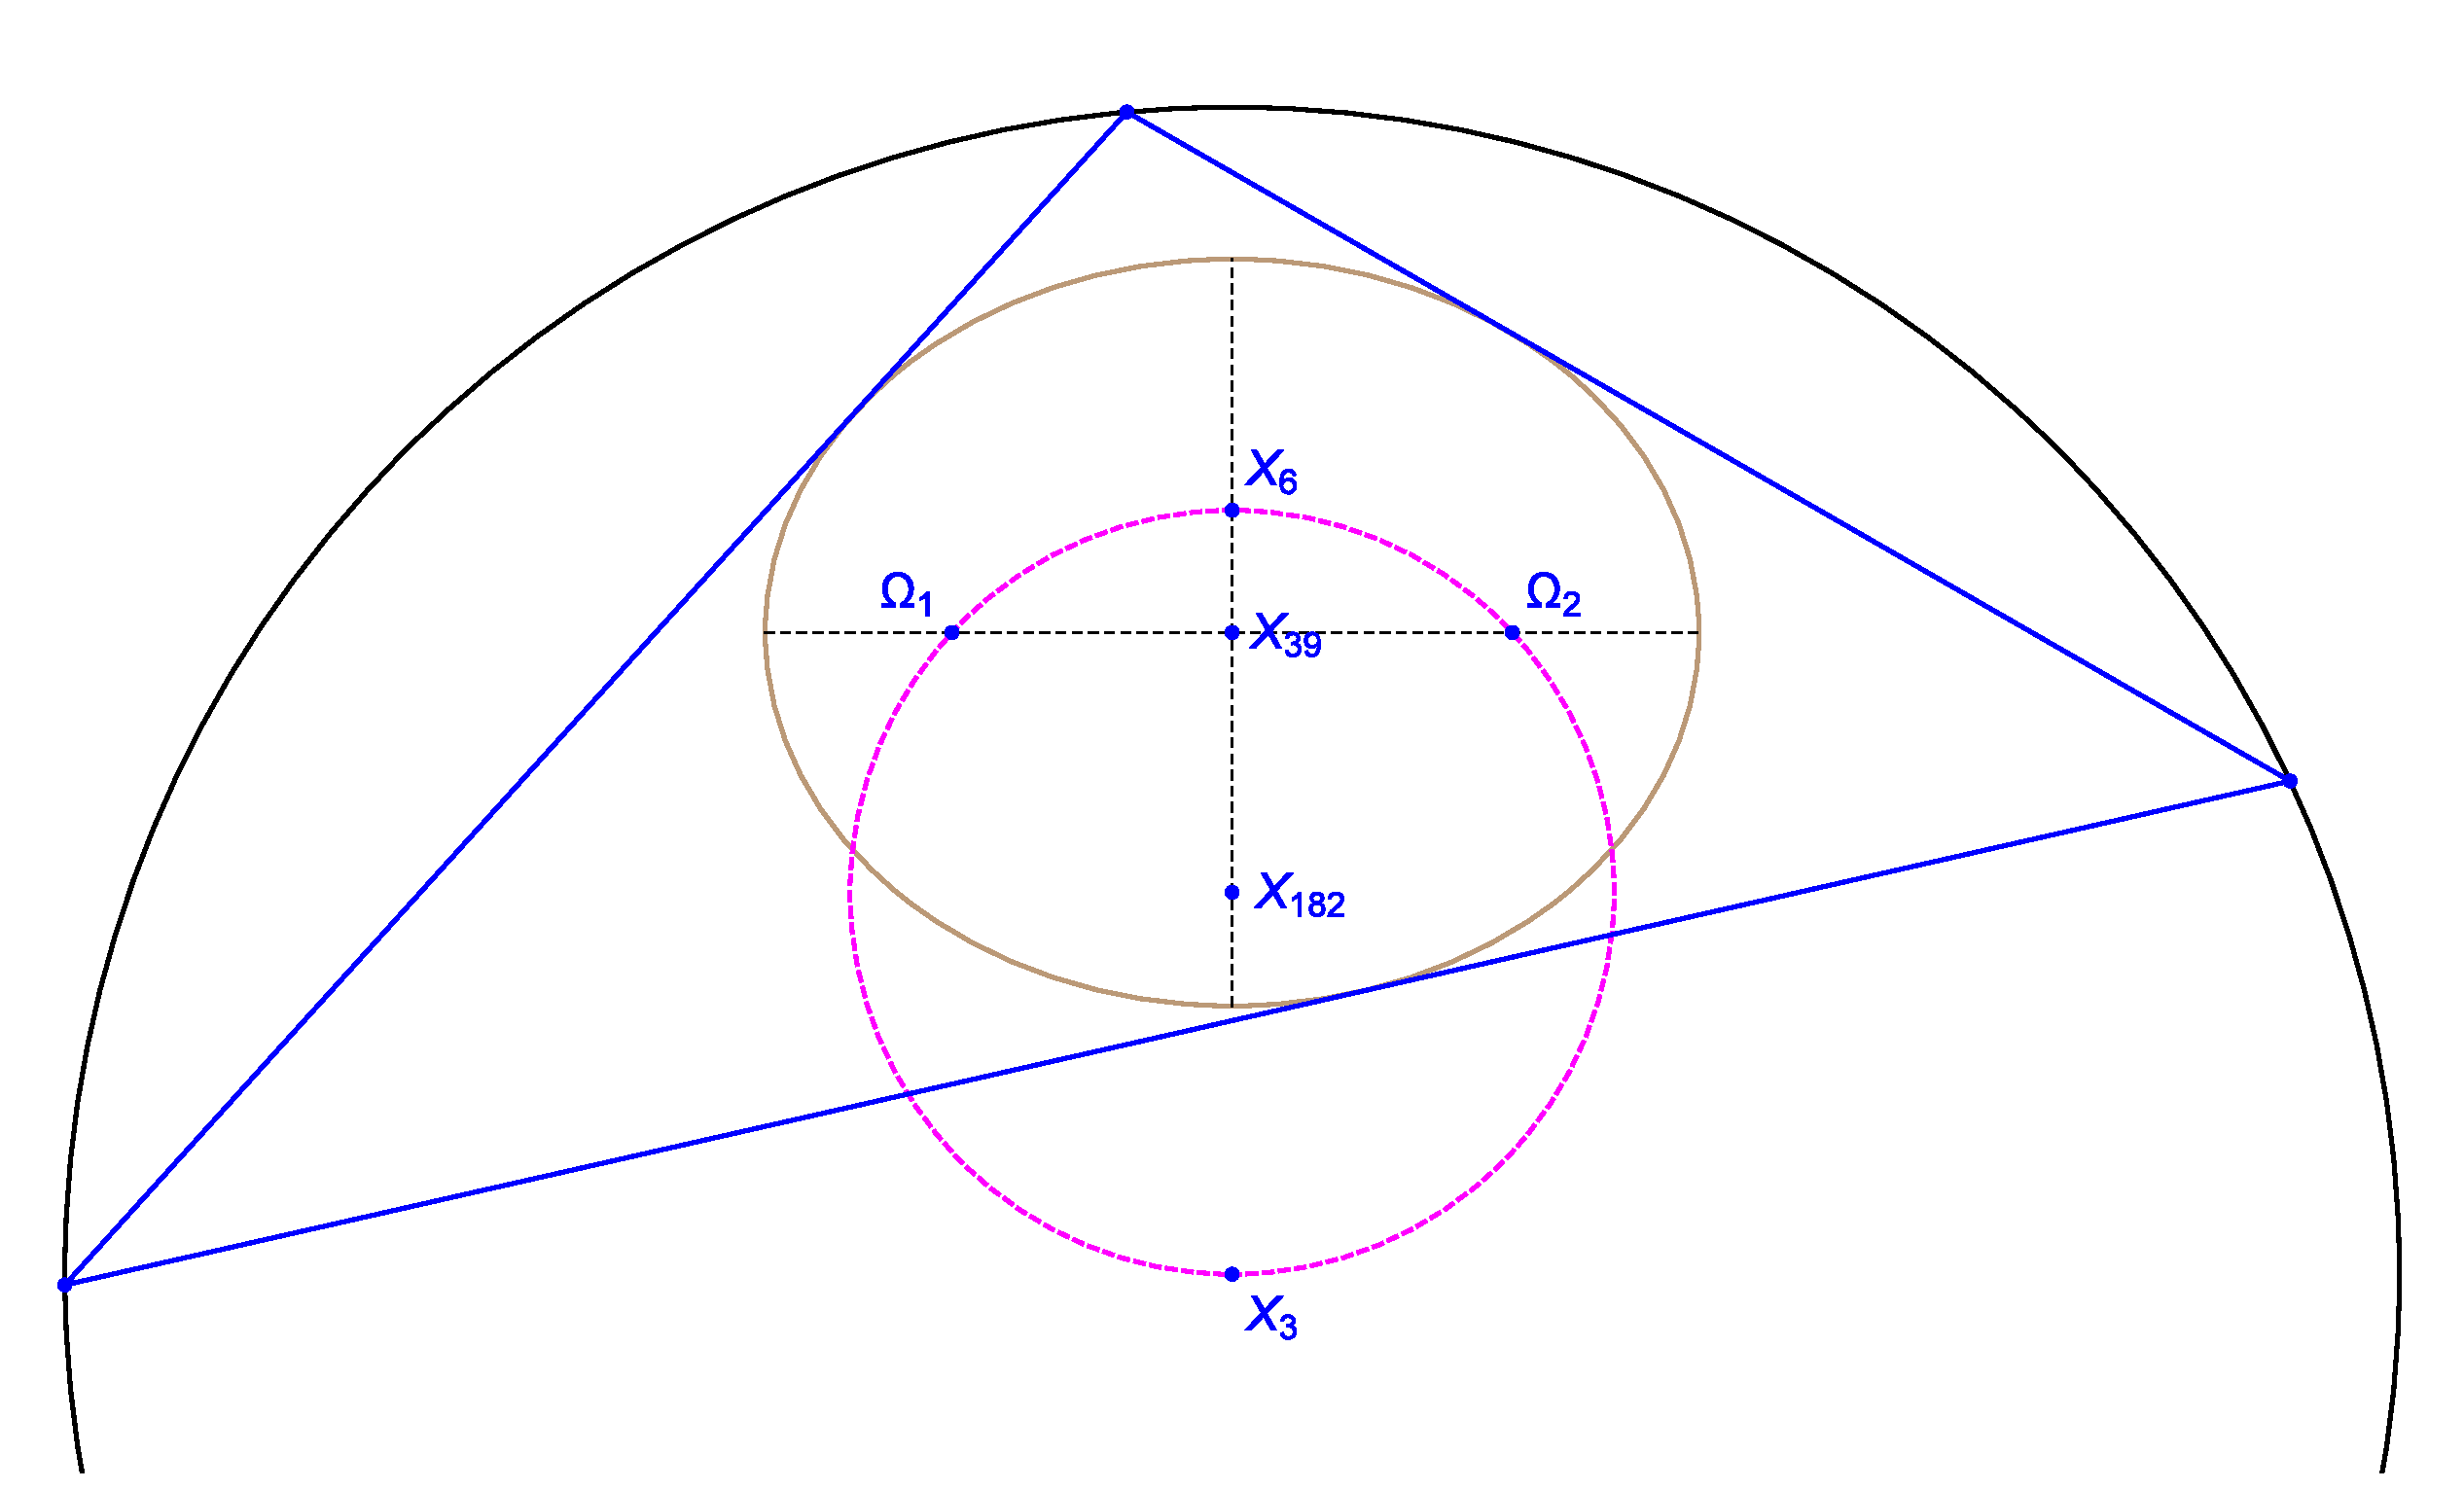
\includegraphics[width=\textwidth]{pics_04_240_brocard_porism}
     \caption{A triangle (blue) in the Brocard porism is shown inscribed in an outer circle (black) and having the Brocard inellipse (brown) as its caustic, with foci at the stationary Brocard points $\Omega_1$ and $\Omega_2$ of the family, and centered on the Brocard midpoint $X_{39}$. The Brocard points as well as the stationary circumcenter $X_3$ and symmedian point $X_6$ are concyclic on the Brocard circle (dashed magenta), whose center is $X_{182}$. \href{https://bit.ly/2QX3lEt}{Live}}
     \label{fig:04-brocard-porism}
 \end{figure}

Referring to \cref{fig:04-brocard-porism}, all of $\Omega_1$, $\Omega_2$, $X_3$, and $X_6$ are concyclic on the so-called Brocard circle, see \cite[Brocard Circle]{mw}, whose center is $X_{182}$. The Brocard axis is defined in \cite[Brocard Axis]{mw} as the line containing the circumcenter $X_3$ and symmedian point $X_6$ of a triangle.
 
\begin{proposition}
Over the Brocard porism, the following 3 objects are stationary: (i) the Brocard circle, (ii) the Brocard axis, and (iii) the symmedian point $X_6$ are stationary.
\label{prop:03-x6-stationary}
\end{proposition}

\begin{proof}
The Brocard circle is stationary since it passes through 3 stationary points: $\Omega_1,\Omega_2,X_3$ are stationary. The Brocard axis is stationary since it contains stationary $X_3$ and stationary Brocard midpoint $X_{39}$. For any triangle, $X_6$ is antipodal to $X_3$ on the Brocard circle.
\end{proof}
 
Recall the two isodynamic points $X_{15}$ and $X_{16}$ of a triangle as the two unique intersections of the 3 Apollonius circles\footnote{These are circles which contain a vertex and the intersection of the corresponding internal and external bisectors with the opposite side.}. $X_{15}$ (resp. $X_{16}$) is interior (resp. exterior) to the circumcircle. In fact they are inverse images of each other with respect to the latter, see \cite[Isodynamic Points]{mw}.

\begin{proposition}
Over the Brocard porism, the two Isodynamic points $X_{15}$ and $X_{16}$ are stationary and given by:

\[
X_{15}=\left[0, \frac{R(\sqrt{3}-\Sha)}{
 \sqrt{\Sha^2-3}}\right],\;\;\;
 X_{16}=\left[0, -\frac{R(\sqrt{3}+\Sha)}{
 \sqrt{\Sha^2-3}}\right]
\]
\label{prop:04-x15x16}
\end{proposition}

\begin{proof}
Let $P$ and $U$ be finite points on a triangle's plane with normalized barycentric coordinates $(p,q,r)$ and $(u,v,w)$, respectively. Let $f$ and $g$ be homogeneous functions of the sidelengths. The $(f,g)$ {\em barycentric combo} of $P$ and $U$, also denoted $f*P + g*U$, is the point with barycentrics $(f\,p + g\,u,f\,q + g\,v, f\,r + g\,w)$. In \cite[X(15), X(16)]{etc}, the following combos (see below), derived by Peter Moses, are provided:

\begin{align}
X_{15} =& \sqrt{3}*X_3 + \Sha*X_6 \label{eqn:combo-x15} \\
X_{16} =& \sqrt{3}*X_3 - \Sha*X_6 \nonumber
\end{align}
 
 With all involved quantities invariant, the result follows.
\end{proof}

\begin{proposition}
The semi-axes $a'$ and $b'$ and center $X_{39}$ of the Brocard inellipse are given by:

\begin{gather*}
[a',b']= R\left[\sin\omega,2\sin^2\omega\right]=R\left[\frac{1}{\sqrt{1+\Sha^2}},\frac{2}{{1+\Sha^2}}\right]\\
 X_{39}=\left[0,-\frac{R\Sha\sqrt{\Sha^2-3}}{\Sha^2+1}\right]
\end{gather*}
 \label{prop:04-brocard-axes}
\end{proposition}

\begin{proof}

Consider a triangle $T$ with sidelengths $s_1,s_2,s_3$, area  $\Delta$, and circumradius  $R$. The following identities appear in \cite{bradley2007-brocard,shail1996-brocard}:

\begin{equation}
R=\frac{s_1 s_2 s_3}{4\Delta}, \;\;\; \sin\omega=\frac{2\Delta}{\sqrt{\Gamma}}
\label{eq:04-broc-R-sinw}
\end{equation}

\noindent where $\Gamma=(s_1 s_2)^2+(s_2 s_3)^2+ (s_3 s_1)^2$. Bringing in \cref{eq:04-omega-dist}, the result follows from combining the above into expressions for the Brocard inellipse semi-axes given in \cite[Brocard Inellipse]{mw}:

\begin{equation}
a' =\frac{s_1 s_2 s_3}{2\sqrt{\Gamma}},\;\;\;\;\;\;b' =\frac{2 s_1 s_2 s_3 \Delta}{\Gamma}
\label{eq:04-broc-axes}
\end{equation}

\end{proof}

With the results above, we can derive the following quantities and centers explicitly:

\begin{align*}
X_6&=\left[0,-\frac{R\sqrt{ \Sha^2 -3}}{ \Sha}\right] \\
|X_3-X_6|&=\frac{R\sqrt{ \Sha^2 -3}}{ \Sha}\\
\Omega_{1,2}(R,\Sha)&=\frac{R\sqrt{ \Sha^2-3}}{ \Sha^2+1} \left[ \pm 1, - \Sha  \right]
%X_{39}&=\left[0,-R {\frac {\Sha\,\sqrt {\Sha^2-3}}{\Sha^2+1}} \right]
\end{align*}

Let $a'$ be the major axis of a generic triangle's Brocard inellipse. Interestingly, we have:

\begin{lemma}
\[ \sum_{i=1}^{3}{\frac{1}{s_i^2}}=\frac{1}{4 (a')^2} \]
\end{lemma}

\begin{proof}
As
\[\frac{1}{s_1^2}+\frac{1}{s_2^2}+\frac{1}{s_3^2}=\frac{s_2^ 2s_3^2+s_1^2 s_3^2+s_1^2 s_2^2}{s_1^2 s_2^2 s_3^2}\]
the result follows from \cref{eq:04-broc-axes}.  
\end{proof}

\noindent Therefore, we have:

\begin{corollary}
Over the Brocard porism, the sum of inverse squared sidelengths is invariant
\end{corollary}

\noindent \textbf{Similarity and Polar image:} As it will be seen below, the Brocard porism is the image of the Homothetic family under two different transformations: variable similarity and polar.

Referring to \cref{fig:04-homot-broc-inell}, we will first prove a handy lemma, introduced in  \cite{reznik2020-similarityII}:

\begin{figure}
    \centering
    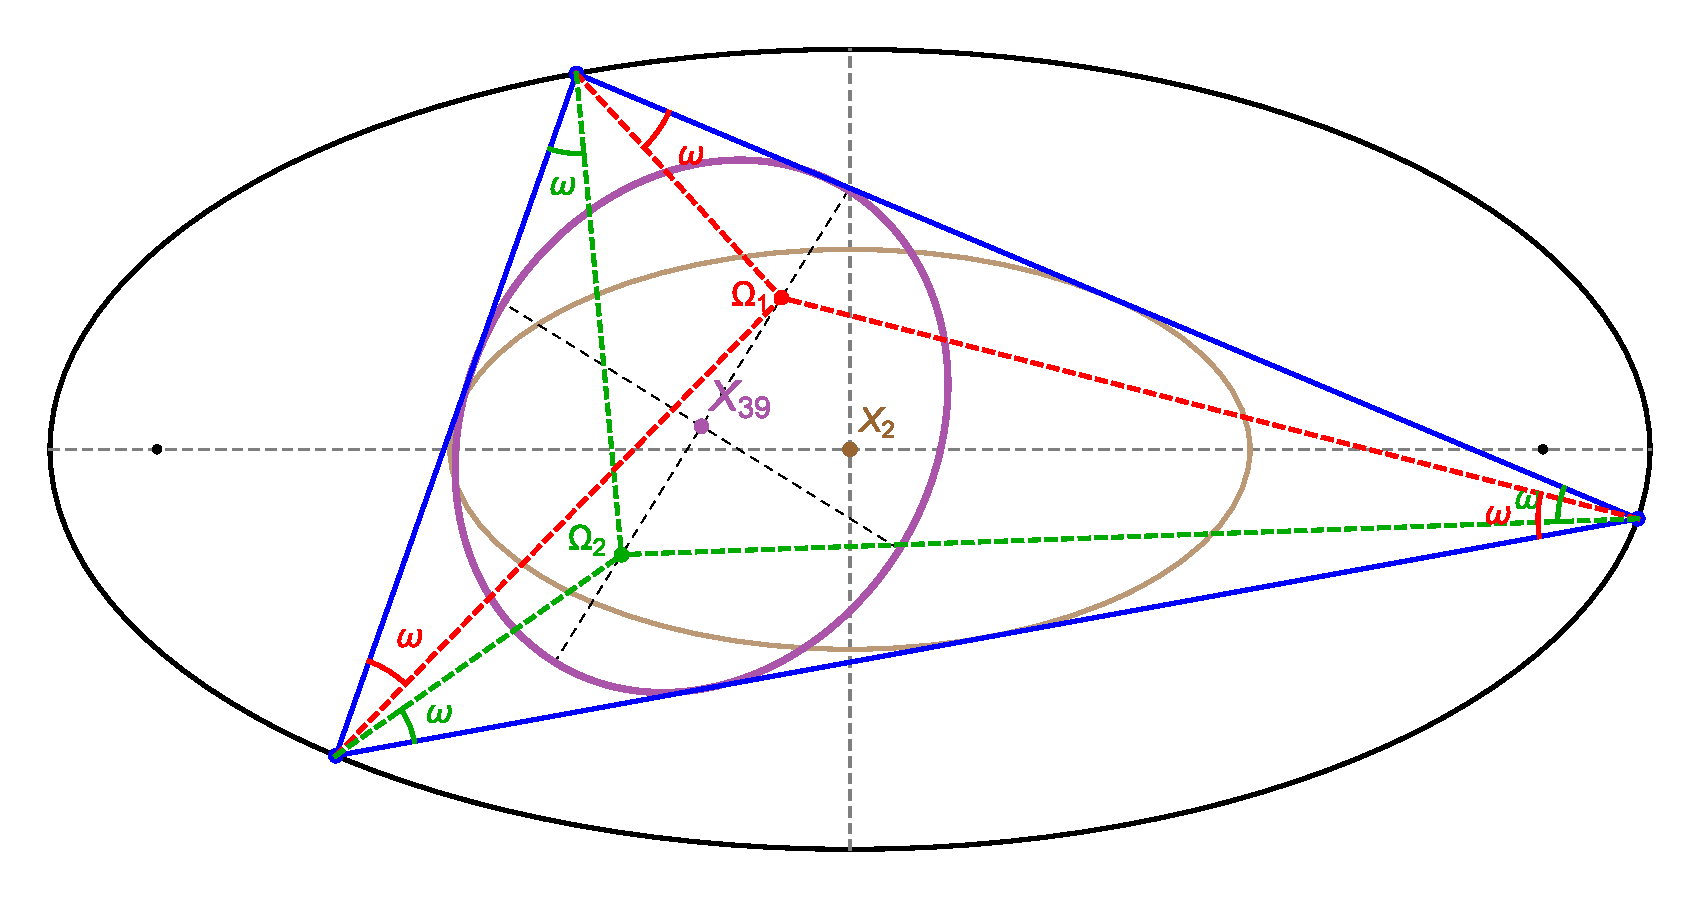
\includegraphics[width=\textwidth]{pics_04_270_homot_broc_inell}
    \caption{Over the homothetic family, the Brocard inellipse has semi-axes of variable lengths but invariant aspect ratio. \href{https://youtu.be/DIm2qTxGWXE}{Video}}
    \label{fig:04-homot-broc-inell}
\end{figure}

\begin{lemma}
Over the homothetic family, though the semi-axes of the Brocard inellipse have variable lengths, their ratio $\beta$ is invariant and given by:
\[\beta=
\frac{\sqrt{3a^4+10a^2b^2+3b^4}}{4ab} > 1\]
\label{lem:04-beta}
\end{lemma}

\begin{proof}
The result follows from combining \cref{eq:04-broc-R-sinw} with \cref{eq:04-broc-axes}, using the sidelengths $s_i$ of the homothetic family using the parametrization in \cref{sec:02-confocal-standard-param}.
\end{proof}

The result below was introduced in \cite[Thm 4.1]{reznik2020-similarityII}:

\begin{proposition}
The Brocard family is the image of the homothetic one under a variable similarity transform.
\end{proposition}

\begin{proof}
Consider the following similarity transform which sends points $X$ in the plane of the homothetic family to new ones $X'$:

\[X'=Scale(1/b'').Rot(-\theta).Transl(-X_{39}).X\]

\noindent where  $b''$ is the variable minor semi-axis length of the the (moving) Brocard inellipse $\E''$ in the homothetic pair, $\theta$ the angle between said minor axis and the horizontal, and $X_{39}$ the moving center of $\E''$. Clearly, $\E''$ will be sent to an origin-centered ellipse which is axis-parallel to the homothetic ones. By Lemma~\ref{lem:04-beta}, the aspect ratio $\beta$ of $\E''$ is invariant over the homothetic family, implying the transformed inellipse will have fixed axes $(\beta, 1)$. Notice its circumcenter and circumradius are prescribed by the semi-axes of the caustic (Equation~\ref{eqn:broc-circumcircle}). This completes the proof. 
\end{proof}

\begin{figure}
    \centering
    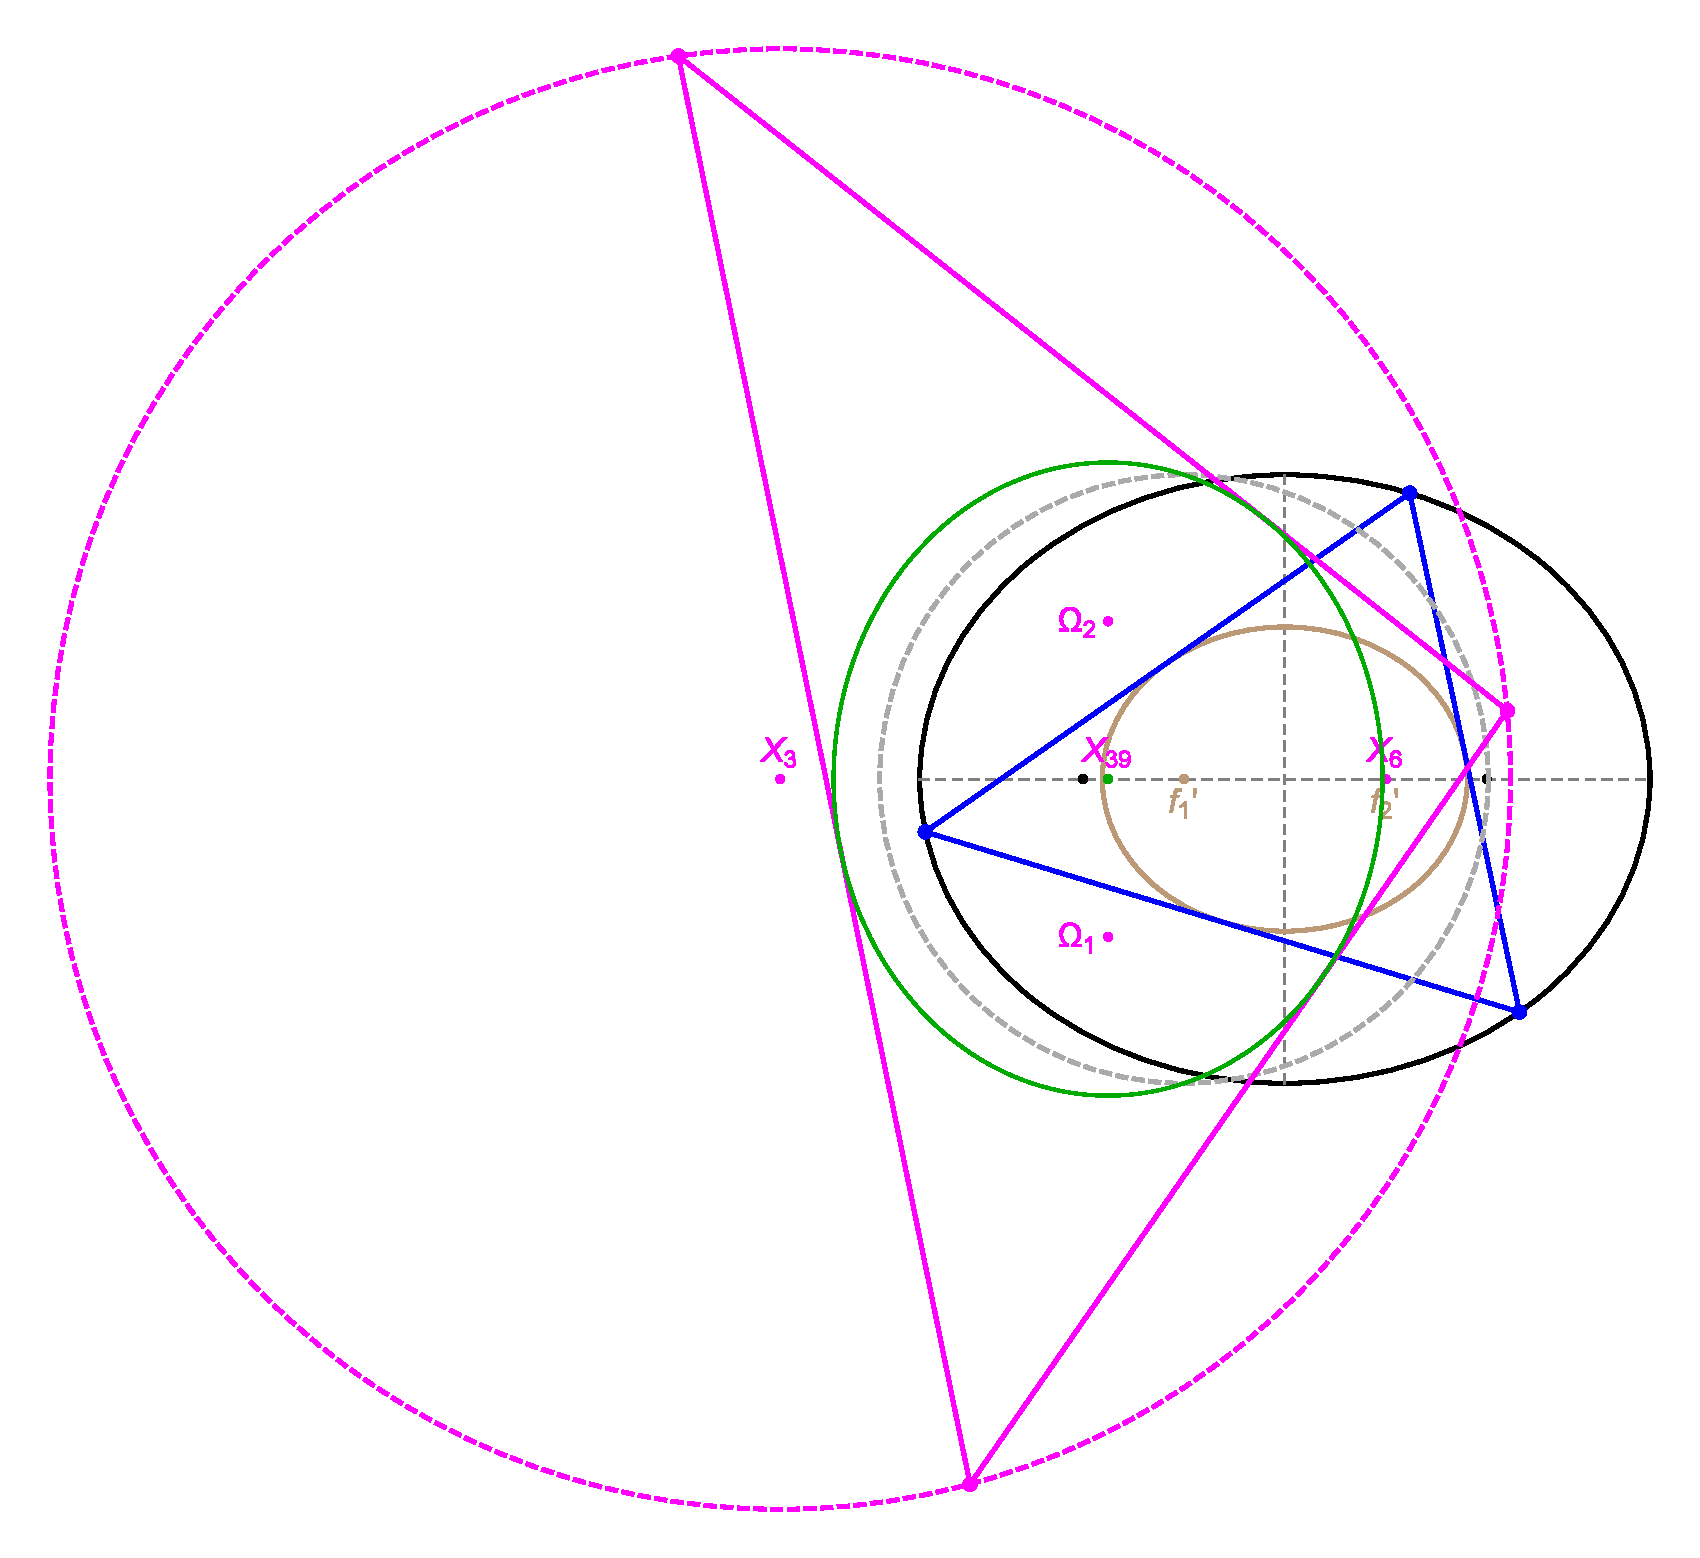
\includegraphics[width=.7\textwidth]{pics_04_260_brocard_homothetic_polar}
    \caption{The Brocard family (magenta) is the polar image of the homothetic family (solid blue) with respect to a circle (dashed gray) centered on a focus of the homothetic caustic (light brown) which is sent to the Brocard circumcircle (dashed magenta). The outer ellipse (black) is sent to the Brocard inellipse (green). \href{https://bit.ly/2RwKmAM}{Live}}
    \label{fig:04-brocard-homoth}
\end{figure}

Referring to \cref{fig:04-brocard-homoth}, let $a,b$ be the semi-axes of the outer ellipse in the homothetic pair. 

\begin{proposition}
The Brocard porism is the polar image of the homothetic family with respect to a circle centered on a caustic focus $f'$.  The symmedian point $X_6$ of the image coincides with $f'$. Its outer circle and ellipse are given by:
\begin{align*}
   \mathcal{C}:&\;\; (x-x_0)^2+y^2  =R^2 \\
  \mathcal{E}:& \;\;  \frac{(x-x_1)^2}{(a')^2}+\frac{y^2}{(b')^2}=1\\
    x_0&=-\frac{c(b^2 + 4\rho^2)}{2b^2},\;\; 
    x_1 =  -\frac{c(4a^2 - c^2 + 4\rho^2)}{2(4a^2 - c^2)}\\
    (a')&= \frac{4a\rho^2}{4a^2 - c^2},\;\;
    (b') = \frac{2a\rho^2 }{b\sqrt{4a^2 - c^2}},\;\; R=\frac{2a\rho^2}{b^2} 
\end{align*}
Here $b'>a'$.
\label{prop:04-brocard-polarimage}
\end{proposition}
 
\begin{proof}
Proof is left as an exercise.
\end{proof}

%%% It follows from the same approach developed in \cref{sec:09-polarimage}.  Details are left to the reader.
\begin{remark}
 From the relations obtained in \cref{prop:04-brocard-polarimage} it follows that
 \[a=\rho^2\frac{(4 (b')^2-(a')^2)}{3 a' (b')^2},\;\; b=\rho^2\frac{\sqrt{4 (b')^2-(a')^2}}{\sqrt{3} (b')^2}\]
 
\end{remark}

Since two polar transformations with respect to the same circle is the identity:

\begin{corollary}
The homothetic family is the polar image of the Brocard family with respect to its stationary symmedian point $X_6$.
\end{corollary}
  
\begin{corollary}
In terms of the homothetic pre-image semi-axes $a,b$, the invariant sum of inverse squared sidelengths and Brocard angle are given by:
 
\begin{align*}
\sum_{i=1}^{3}{\frac{1}{s_i^2}}&=\frac{1}{4 (b')^2}=\frac{b^2(3a^2 + b^2)}{ 16\rho^4a^2}  \\
 \cot\omega&=\Sha=\sqrt{3}\frac{a }{b } 
\end{align*}
\end{corollary}

\begin{proof} By \cref{prop:04-brocard-axes} and \cref{prop:04-brocard-polarimage} it follows that
  $\sin\omega=(a')/(2b')=b/\sqrt{4a^2-c^2}.$
Using that $\csc^2\omega-\cot^2\omega=1$ the result follows.
\end{proof}

\subsection{A digression: Equilateral Isodynamic Pedals}
\label{sec:04-brocard-isodyn-pedals}

Referring to Figure~\ref{fig:04-isodynamic-equis}, the pedal (resp. antipedal) triangles of the isodynamic points $X_{15}$ and $X_{16}$ (resp. isogonic points $X_{13}$ and $X_{14}$) are equilaterals centered on $X_{396}$ and $X_{395}$ (resp.  $X_{5463}$ and $X_{5464}$) \cite{etc}.

Let $A$ denote the area of a triangle and $A_k$, $k={13,14,15,16}$ denote the area of said equilaterals. \cite{moses2020-private-equilaterals} has kindly contributed the following expressions:

\begin{proposition}
\begin{align*}
A_{13}/A =& 2 + \frac{2 \Sha}{\sqrt{3}},\;\;\;A_{14}/A = 2 - \frac{2 \Sha}{\sqrt{3}}\\
A_{15}/A =& \frac{-3 + \sqrt{3} \Sha}{2(\csc^2\omega - 4)},\;\;\;
A_{16}/A = \frac{-3 - \sqrt{3} \Sha}{2(\csc^2\omega - 4)}
\end{align*}
\label{prop:04-equi-areas}
\end{proposition}


\begin{corollary}
For any triangle:
\[ \frac{A_{13}}{A_{14}}=\frac{A_{16}}{A_{15}}= \frac{\Sha+\sqrt{3}}{\Sha -\sqrt{3}} \]
\end{corollary}

\begin{corollary}
The Brocard porism conserves $A_{13}/A_{14}$ and $A_{16}/A_{15}$.
\end{corollary}

%\[
%\frac{A_{16}}{A_{15}}= {\frac { \left( s_1^{2}+s_2^{2}+s_3^{2} \right)  \left( s_1^{2}+s_2^{2}+s_3^{2}+2\,2\sqrt {3}A \right) }{2\,s_1^{4}-2\,s_1^{2}s_2^{2}-2\,s_1^{2}s_3^{2}+2\,s_2^{4}-2\,s_2^{2}s_3^{2}+2\,s_3^{4}}}-1\]

%Using Conwayng the above over the Brocard porism vertices (Proposition~\ref{prop:orbita}) and using a CAS for simplication obtain:

%\[\frac{A_{16}}{A_{15}}= \frac{(\sqrt{3}h-3d)^2}{(\sqrt{3}h+3d)^2}\]

%A further simplification using Lemma \ref{lem:7} leads to the result.
%\end{proof}

\begin{figure}
    \centering
    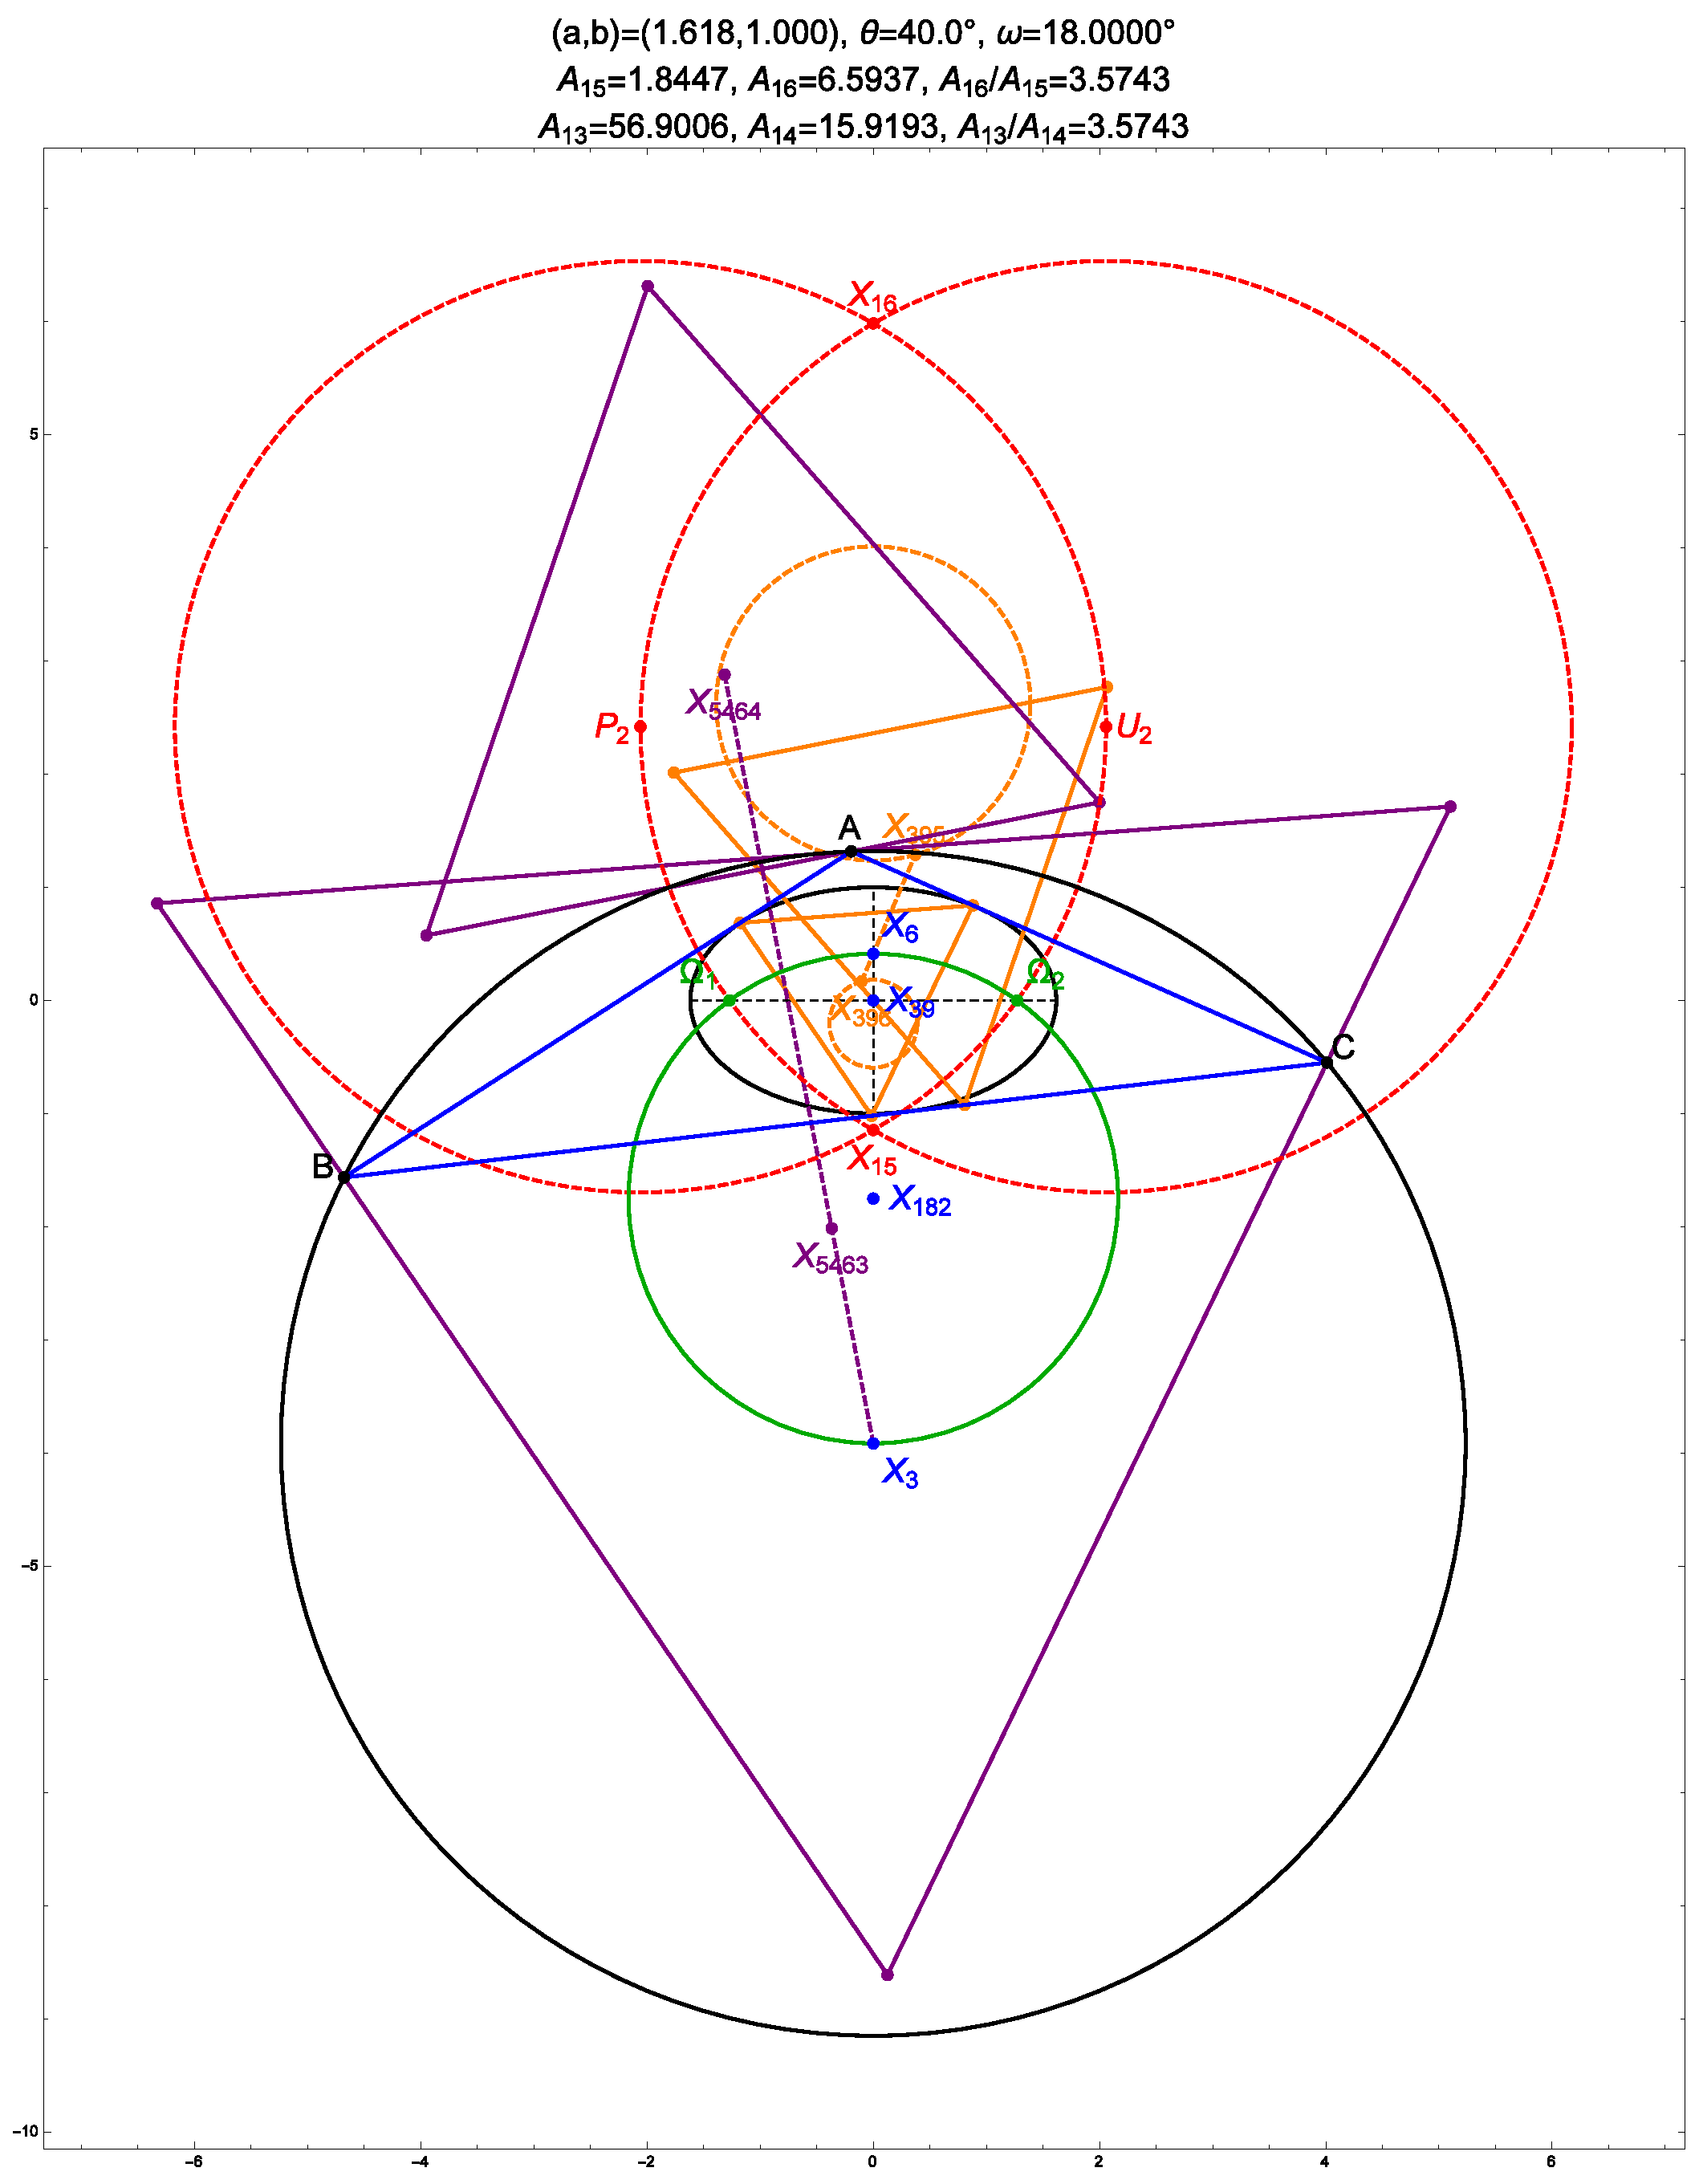
\includegraphics[width=\textwidth]{pics_04_280_broc_isos.eps}
    \caption{The pedal (resp. antipedal) triangles (orange, resp. purple) of the isodynamic points $X_{15}$ and $X_{16}$ (resp. isogonic points $X_{13}$ and $X_{14}$) are equilaterals centered on $X_{396}$ and $X_{395}$, collinear with $X_6$ (resp. $X_{5463}$ and $X_{5464}$, collinear with $X_3$) \cite{etc}. Over the porism, the area ratios $A_{16}/A_{15}$ and $A_{13}/A_{14}$ are invariant and identical. The loci of $X_{396}$ and $X_{395}$ are circles (dashed orange) as are those of $X_{5463}$ and $X_{5464}$ (not shown).
    \href{https://youtu.be/s4DF-iZZO8Y}{Video}}
    \label{fig:04-isodynamic-equis}
\end{figure}

The centroid of the pedal triangle of $X_{15}$ (resp. $X_{16}$) is  $X_{396}$ (resp. $X_{395}$).


\begin{proposition}
The locus of $X_{15}$ and $X_{16}$ pedal centroids $X_{396}$ and $X_{395}$ are the following circles:

\[C_{395}= \left[ 0,  \frac {R \left(  3(\Sha^2+1)-2\,\sqrt {3}\;\Sha \right) 
 \left( \Sha+ \sqrt {3} \right) }{3\sqrt { \Sha^2-3} \left(  
\Sha^2+1 \right) }
 \right],\;\;
r_{395}=\frac{R (\sqrt{3}\Sha +3)}{3(\Sha^2+1)}\]
\[C_{396}= \left[ 0,  \frac {R \left(3\, ( \Sha^2+1 )+ 2\,\sqrt {3}\;\Sha \right) 
 \left(  \Sha -\sqrt {3}\right) }{3\sqrt {\Sha^2-3} \left( \Sha^{2}+1 \right) }
 \right],\;\;
r_{396}=\frac{R (\sqrt{3}\Sha -3)}{3(\Sha^2+1)}\]

\end{proposition}

\begin{proof}
Obtained via CAS.
\end{proof}

\begin{remark}
Notice the ratio $r_{395}/r_{396}$ is equal to $A_{396}/A_{395}$.
\end{remark}

Still referring to \cref{fig:04-isodynamic-equis}:

\begin{proposition}
The locus of $X_{13}$ and $X_{14}$ antipedal centroids $X_{5463}$ and $X_{5464}$ are the following circles:
\end{proposition}


\section{Vertex Parametrization}

\subsection{Poristic family}
\label{sec:04-vtx-poristic}

Consider a pair of circles $x^2+y^2=R^2$,
$(x-d)^2+y^2=r^2$, with $d^2=R(R-2r)$. Then a 3-periodic orbit is parametrized by:

\begin{align}
P_1&=[x_1,y_1]\nonumber \\
 P_2&=\frac{1}{w^2} [ -4R r^2 q  y_1 - w_1w_2 , -2r R w_1y_1 + 2 r q w_2 ]\nonumber \\
  P_3 &=  \frac{1}{w^2} [4R r^2 q  y_1 - w_1w_2 , -2r R w_1y_1 - 2 r q w_2 ]\label{eq:04-vtx-poristic} \\
  q&=\sqrt{R^2 - r^2 - 2d x_1  + d^2},\;\; w=R^2 - 2d x_1  + d^2\nonumber 
  \\ w_1&=R^2 - 2r^2 - 2 d x_1 + d^2,\;\;\;
  w_2=(R^2+d^2) x_1 - 2 R^2 d  \nonumber
\end{align}

\subsection{Poristic Excentrals}

Its vertices sweep a circle centered on $X_{40}$ of the original poristic family, so we omit the parametrization.

\subsection{Brocard Porism}
\label{sec:04-broc-porism}

Consider an isosceles Poncelet triangle $\Tm=ABC$ in the Brocard porism, where $AB$ is tangent to $\E$ at one of its minor vertices. Let $|AB|=2d$ and the height be $h$. Let $\zeta=d^2+h^2$. Let the origin $(0,0)$ be at its circumcenter $X_3$. Its vertices will be given by:

\[A=\left[-d ,\frac{d^2-h^2}{2h}\right], \;\;\; B= \left[d,\frac{d^2-h^2}{2h}\right], \;\;\; \left[0 ,\frac{\zeta}{2h}\right] \]


\begin{proposition}\label{prop:pair_brocard}
The Brocard porism containing $\Tm$ as a Poncelet triangle is defined by the following circumcircle $\K_0$ and Brocard inellipse $\E$:

\begin{align*}
\K_0:&\, x^2+y^2-R^2=0, \;\;\; R=\frac{\zeta}{2h}\\
\E:&\, -64d^2  h^4  x^2-4  h^2  (9  d^2+h^2)  \zeta  y^2 +4  h  (3  d^2+h^2)  (3  d^2-h^2)  \zeta  y\\&-(d^2-h^2) (9d^2 -h^2) \zeta^2=0
\end{align*}
\end{proposition}

\begin{proof}
The proof follows from $\Tm$, and isosceles Poncelet triangle. Recall that the Brocard inellipse is centered at $X_{39}$. Its perspector is $X_6$, i.e., it will be tangent to $\Tm$ where cevians through $X_6$ intersect it; see \cite[Brocard inellipse]{mw}.
\end{proof}

Consider the pair: circle $x^2+y^2=R^2=(d^2+h^2)^2/(4h^2)$ and   ellipse
$x^2/a^2+(y-y_0)^2/b^2=1$, with  semi-axes
 \[  (a,b)=\left(\frac{d\sqrt{d^2+h^2}}{9d^2+h^2},\frac{4d^2}{9d^2+h^2}\right)
    \]
and center $(0,y_0)$,  $y_0=(9d^4 - h^4)/(2h(9d^2  +  h^3))$.

Vertices $P_i=[x_i,y_i]$, $i=1,2,3$ of Brocard porism triangles are given by:

{\small  
\begin{equation}
    \aligned
    x_1 &= \cos{t}/q_1\\
    y_1 &= \sin{t}/q_1 \\
    x_2 &= -d (d^2 + h^2) ((3 d^2 + h^2)\sin{t} + 2d h \cos{t}- 3 d^2 + h^2)/q_2 \\
    y_2&=-(d^2 + h^2) ((9 d^4 - 2 d^2 h^2 + h^4)\sin{t} - 2 d h (3 d^2 + h^2)\cos{t} - 9 d^4 + h^4)/(2 b q_2) \\
    x_3 &= d (d^2 + h^2) (2 d h \cos{t} - (3 d^2 + h^2) \sin{t} + 3 d^2 - h^2)/q_3\\
    y_3 &=(d^2 + h^2) (2d h (3 d^2 + h^2) \cos{t}+ (9 d^4 - 2 d^2 h^2 + h^4)\sin{t} - 9 d^4 + h^4)/(2 b q_3) \\
    q_1&=(2h)/(d^2+h^2)\\
    q_2&= 2 d h (3 d^2 - h^2)\cos{t} - (9 d^4 - h^4) \sin{t}  + 9 d^4 + 2 d^2 h^2 + h^4\\
    q_3&= 2 d h (3 d^2 - h^2)\cos{t} + (9 d^4 - h^4)\sin{t} - 9 d^4 - 2 d^2 h^2 - h^4
\endaligned
\label{eqn:04-vertices-brocard}
\end{equation}
}



